%% ==============================
\chapter{Implementierung}
\label{cha:implementierung}
%% ==============================

Das vorangegangene Kapitel hat die HCS-basierte Ledger-Schicht entworfen und ein Evaluationskonzept festgelegt, das an mehreren Stellen ausdrücklich auf dieses Kapitel verweist: die Knotenanzahl und die Ausführungsumgebung (Abschnitt~\ref{subsec:eval-aufbau}), die Grundlast (Abschnitt~\ref{subsec:eval-szenarien}) sowie die Symmetriebedingung für den Widerruf (Abschnitt~\ref{subsec:eval-validitaet}). Dieses Kapitel löst diese Festlegungen ein und beschreibt den Aufbau, mit dem die Evaluation durchgeführt wird.

Für die Abgrenzung gegenüber Kapitel~\ref{sec:results} gilt dabei ein durchgehendes Kriterium: In diesem Kapitel werden Messwerte nur dort berichtet, wo sie eine Konstruktions- oder Betriebsentscheidung des Aufbaus begründen, etwa den Nachweis der symmetrischen Messgrenze oder die Begründung der Ein-Arm-Regel. Alle Werte, die Gegenstand der Evaluation selbst sind, einschließlich der Vorabmessungen zur Messmethodik, werden in Kapitel~\ref{sec:results} berichtet. Die hier beschriebenen Verfahren verweisen deshalb an mehreren Stellen auf dieses Kapitel vorwärts.


\section{Überblick und Abgrenzung des Messaufbaus}
\label{sec:impl-ueberblick}

Der Messaufbau realisiert nicht die vollständige Referenzarchitektur, sondern genau denjenigen Ausschnitt, der innerhalb der in Abschnitt~\ref{subsec:eval-aufbau} festgelegten Messgrenze liegt. Betrieben werden je Variante ein einzelner Aries-Agent und die zugehörige Ledger-Infrastruktur; die Anwendungskomponenten der Referenzarchitektur, insbesondere der Konnektor und die Halter-Anwendungen, sind nicht Bestandteil des Aufbaus. Diese Reduktion folgt unmittelbar aus dem Evaluationskonzept: Die Last wird ausschließlich über die Verifiable-Data-Registry-Schnittstelle erzeugt, sodass die DIDComm-Protokolle der Agentenschicht nicht in die Messung eingehen. Ein vollständiger Anwendungsstapel würde diese Protokolle einbeziehen und damit genau die Zuordenbarkeit gemessener Unterschiede zur Ledger-Schicht aufheben, die Abschnitt~\ref{subsec:abgrenzung} als Begründung der Abgrenzung anführt.

Der Agent wird in beiden Varianten aus demselben Basisabbild und mit derselben Konfiguration betrieben; unterschiedlich ist ausschließlich die geladene Registry-Implementierung und die dahinterliegende Ledger-Infrastruktur. Die Schreib- und Leseoperationen werden über die \texttt{/anoncreds/*}-Endpunkte des Agenten ausgelöst, die in beiden Varianten identisch sind. Damit liegt die Messgrenze nicht an einer nachträglich gezogenen Linie, sondern an einer im Agenten tatsächlich vorhandenen Abstraktionsschicht, deren Symmetrie in Abschnitt~\ref{sec:impl-symmetrie} nachgewiesen wird.

\begin{figure}[H]
    \centering
    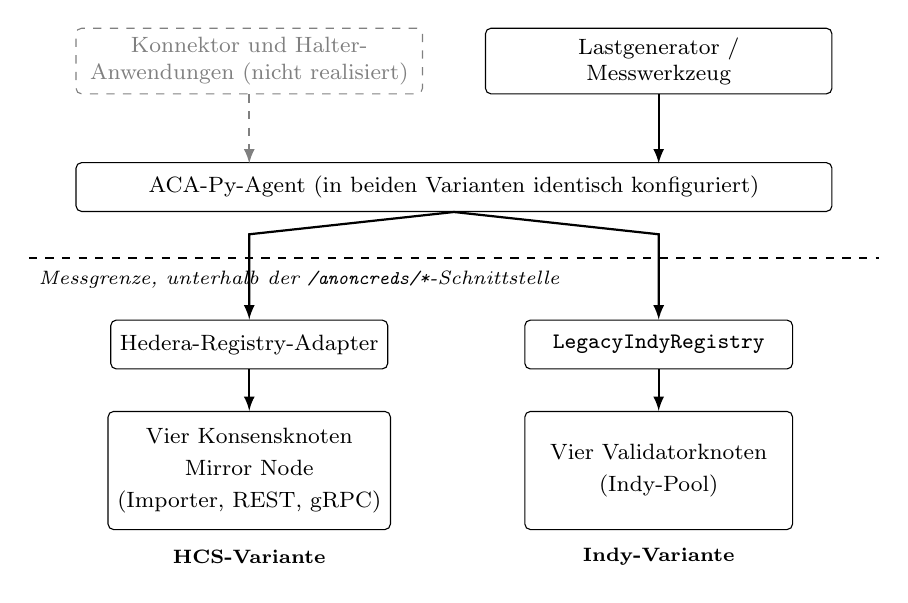
\begin{tikzpicture}[
      font=\footnotesize,
      box/.style={draw, rounded corners=2pt, minimum width=3.4cm, minimum height=0.62cm, align=center},
      ausgegraut/.style={box, draw=gray, text=gray, dashed},
      pfeil/.style={-latex, thick}
    ]
      \node[ausgegraut, minimum width=4.4cm] (nichtreal) at (-2.6,0) {Konnektor und Halter-\\Anwendungen (nicht realisiert)};
      \node[box, minimum width=4.4cm] (last) at (2.6,0) {Lastgenerator /\\Messwerkzeug};
      \node[box, minimum width=9.6cm] (agent) at (0,-1.6) {ACA-Py-Agent (in beiden Varianten identisch konfiguriert)};
      \draw[pfeil] (last) -- (2.6,-1.3);
      \draw[pfeil, gray, dashed] (nichtreal) -- (-2.6,-1.3);
      \draw[dashed, thick] (-5.4,-2.5) -- (5.4,-2.5);
      \node[anchor=west, font=\scriptsize\itshape] at (-5.4,-2.78) {Messgrenze, unterhalb der \texttt{/anoncreds/*}-Schnittstelle};
      \node[box] (adapterh) at (-2.6,-3.6) {Hedera-Registry-Adapter};
      \node[box] (adapteri) at (2.6,-3.6) {\texttt{LegacyIndyRegistry}};
      \node[box, minimum height=1.5cm] (ledgerh) at (-2.6,-5.2) {Vier Konsensknoten\\[2pt] Mirror Node\\[2pt] (Importer, REST, gRPC)};
      \node[box, minimum height=1.5cm] (ledgeri) at (2.6,-5.2) {Vier Validatorknoten\\[2pt] (Indy-Pool)};
      \draw[pfeil] (agent.south) -- (-2.6,-2.2) -- (adapterh);
      \draw[pfeil] (agent.south) -- (2.6,-2.2) -- (adapteri);
      \draw[pfeil] (adapterh) -- (ledgerh);
      \draw[pfeil] (adapteri) -- (ledgeri);
      \node[font=\scriptsize\bfseries] at (-2.6,-6.3) {HCS-Variante};
      \node[font=\scriptsize\bfseries] at (2.6,-6.3) {Indy-Variante};
    \end{tikzpicture}
    \caption{Messaufbau beider Varianten. Innerhalb der gestrichelten Messgrenze liegen der Registry-Adapter und die Ledger-Infrastruktur; der Agent und der Lastgenerator liegen außerhalb. Die Anwendungskomponenten der Referenzarchitektur sind nicht realisiert. Es wird stets nur eine der beiden Varianten betrieben (Abschnitt~\ref{sec:impl-betrieb}).}
    \label{fig:messaufbau}
\end{figure}

Die Tabelle~\ref{tab:impl-komponenten} ordnet den in Abschnitt~\ref{subsec:zielarchitektur-komponenten} beschriebenen Komponenten der Zielarchitektur ihre konkrete Umsetzung zu und weist aus, welche Komponenten im Messaufbau bewusst nicht realisiert sind.

\begin{table}[htbp]
\renewcommand{\arraystretch}{1.3}
\footnotesize
  \centering
  \caption{Umsetzung der Komponenten der Zielarchitektur im Messaufbau}
  \label{tab:impl-komponenten}
  \begin{tabular}{p{0.22\textwidth} p{0.48\textwidth} p{0.20\textwidth}}
    \toprule
    \textbf{Komponente} & \textbf{Umsetzung im Messaufbau} & \textbf{Lage zur Messgrenze} \\
    \midrule
    Konsensnetzwerk & Vier Konsensknoten, lokal betrieben (Abschnitt~\ref{subsec:impl-hcs-netzwerk}) & innerhalb \\
    Mirror Node & Selbst betriebene Mirror Node mit Importer, REST- und gRPC-Schnittstelle & innerhalb \\
    Topics & Zur Laufzeit angelegt; je Objekt ein Topic mit einzelnem \texttt{submitKey} des Ausstellers; kein separates Vertrauens-Topic (Abschnitt~\ref{sec:impl-befunde}, Befund B4) & innerhalb \\
    Registry-Adapter & ACA-Py-Erweiterung für Hedera, geladen über die Erweiterungsschnittstelle (E7) & innerhalb \\
    Agentenschicht & Ein einzelner ACA-Py-Agent, unverändert, in beiden Varianten identisch konfiguriert & außerhalb \\
    Konnektor und Halter-Anwendungen & Nicht realisiert; Last wird direkt über die Registry-Schnittstelle erzeugt & außerhalb \\
    \bottomrule
  \end{tabular}
\end{table}
\normalsize


\section{Umsetzung der HCS-basierten Variante}
\label{sec:impl-hcs}

\subsection{Komponenten und Versionsstand}
\label{subsec:impl-hcs-komponenten}

Die Anbindung der Ledger-Schicht erfolgt nach Entscheidung E7 über die bestehende Hedera-Erweiterung für ACA-Py~\cite{acapyhedera}, die sich in die \texttt{AnonCredsRegistry}-Schnittstelle des Agenten einhängt. Der Versionsstand ist dabei nicht frei wählbar, sondern durch eine Verträglichkeitsbedingung bestimmt: Die Erweiterung ist jeweils gegen einen bestimmten Stand des Agenten entwickelt, und die von ihr benötigten \texttt{/anoncreds/*}-Endpunkte stehen nur bei einem bestimmten Wallet-Typ zur Verfügung. Festgelegt wurde daher die Kombination aus ACA-Py in der Version 1.3.0, der auf denselben Stand ausgelegten Erweiterung und dem Wallet-Typ \texttt{askar-anoncreds}. Diese Kombination wurde vor Beginn der Messungen als funktionsfähig nachgewiesen und über den gesamten Messzeitraum unverändert gehalten.

Diese Festlegung hat eine methodische Konsequenz, die hier festzuhalten ist: Der Messaufbau ist damit von der parallel laufenden Modernisierung der Referenzimplementierung entkoppelt. Die Evaluation misst einen fixierten, vollständig dokumentierten Softwarestand und nicht einen sich während der Messreihe verändernden Entwicklungsstand. Der Preis dieser Entkopplung ist, dass der gemessene Stand nicht notwendigerweise der jeweils aktuellste ist; dies wird in Abschnitt~\ref{sec:impl-grenzen} als Gültigkeitsgrenze geführt.

Die Kopplung zwischen Wallet-Typ und verfügbaren Schnittstellen ist dabei kein Konfigurationsdetail, sondern eine strukturelle Eigenschaft des Agenten mit unmittelbarer Auswirkung auf die Messgrenze. Sie wird in Abschnitt~\ref{sec:impl-befunde} als eigenständiger Implementierungsbefund berichtet, da sie beim Aufbau zu einem stillen Fehlzustand führen kann.

\begin{table}[htbp]
\renewcommand{\arraystretch}{1.3}
\footnotesize
  \centering
  \caption{Fixierter Versionsstand beider Varianten}
  \label{tab:impl-versionsstand}
  \begin{tabular}{p{0.26\textwidth} p{0.34\textwidth} p{0.30\textwidth}}
    \toprule
    \textbf{Bestandteil} & \textbf{HCS-Variante} & \textbf{Indy-Variante} \\
    \midrule
    Basisabbild des Agenten & \texttt{acapy-agent:py3.12-1.3.0} & identisch \\
    ACA-Py & 1.3.0 & 1.3.0 \\
    Wallet-Typ & \texttt{askar-anoncreds} & \texttt{askar-anoncreds} \\
    Registry-Implementierung & Hedera-Erweiterung, Stand 1.3.0, auf Commit festgelegt~\cite{acapyhedera} & \texttt{LegacyIndyRegistry} (Bestandteil von ACA-Py) \\
    Ledger-Bibliothek & \texttt{hiero-did-sdk-python} 0.1.0 (angepasst, Abschnitt~\ref{subsec:impl-hcs-patch}), \texttt{hiero\_sdk\_python} 0.1.1 & \texttt{indy-vdr} 0.4.2 \\
    Netzwerk & Vier Konsensknoten, selbst betrieben, mit Mirror Node & Vier Validatorknoten, selbst betrieben \\
    \bottomrule
  \end{tabular}
\end{table}
\normalsize
Die Tabelle weist den Stand der Agentenschicht aus. Der Stand der Indy-Knoten selbst ist damit nicht abgedeckt und wird getrennt in Abschnitt~\ref{subsec:impl-indy-netzwerk} ausgewiesen, wo zugleich eine Einschränkung seiner Nachvollziehbarkeit festzuhalten ist.


\subsection{Konsensnetzwerk und Mirror Node}
\label{subsec:impl-hcs-netzwerk}

Entscheidung E1 verlangt ein selbst betriebenes, mehrknotiges Hashgraph-Netzwerk. Umgesetzt wird dies mit dem containerisierten, Kubernetes-basierten Bereitstellungswerkzeug des Hedera-Ökosystems, das ein vollständiges Netzwerk aus Konsensknoten und Mirror Node lokal erzeugt~\cite{hierosolo}. Die Knotenanzahl wird auf vier festgelegt, womit nach dem aBFT-Modell des Hashgraph-Konsens eine Fehlertoleranz von einem byzantinischen Knoten erreicht wird~\cite{bairdgross2019}; diese Festlegung löst die in Abschnitt~\ref{subsec:eval-aufbau} offen gelassene Dimensionierung ein und ist Voraussetzung für das Szenario S4.

Der Aufbau des Netzwerks erfolgt nicht über den vom Werkzeug angebotenen Einschrittbefehl, sondern über den vollständigen, aus Einzelschritten bestehenden Ablauf. Der Grund ist ein Verhalten des Werkzeugs in der eingesetzten Version, das während des Aufbaus festgestellt wurde: Der Einschrittbefehl nimmt die gewünschte Knotenanzahl als Parameter entgegen, gibt sie im eigenen Protokoll zurück und meldet einen erfolgreichen Abschluss, stellt jedoch tatsächlich nur einen einzigen Konsensknoten bereit. Der Parameter wird also ohne Fehlermeldung verworfen. Da eine falsche Knotenanzahl die Vergleichbarkeit mit der Indy-Variante nach NFA6 unmittelbar aufheben würde und der Fehlzustand aus dem Protokoll des Werkzeugs nicht erkennbar ist, wird der mehrschrittige Ablauf verwendet und die tatsächliche Knotenanzahl nach jedem Aufbau eigenständig verifiziert.

\begin{lstlisting}[basicstyle=\ttfamily\footnotesize, frame=single, caption={Ablauf des Netzwerkaufbaus mit vier Konsensknoten}, label={lst:solo-flow}]
1. Kubernetes-Cluster erzeugen
2. Werkzeug initialisieren, Cluster-Referenz verbinden und einrichten
3. Deployment anlegen
4. Cluster mit Knotenanzahl 4 an das Deployment binden
5. Gossip- und TLS-Schluessel fuer alle Knoten erzeugen
6. Konsensnetzwerk ausrollen
7. Knoten einrichten und starten
8. Mirror Node mit angepasster Wertedatei hinzufuegen
\end{lstlisting}

Schritt 5 ist dabei derjenige Schritt, dessen Auslassung am ehesten unbemerkt bleibt: Ohne erzeugte Schlüssel scheitert erst das Ausrollen in Schritt 6, und zwar mit einer Meldung, die nicht auf die fehlenden Schlüssel verweist. Die Verifikation des erreichten Zustands erfolgt nicht über die Bereitschaftsanzeige der Container, da diese bereits vor der Betriebsbereitschaft der Konsensplattform gesetzt wird, sondern über den im Protokoll der Plattform ausgewiesenen Zustand sowie über die Übereinstimmung aller vier Knoten auf derselben Konsensrunde.

Für die Mirror Node sind zwei Eigenschaften für die spätere Messung wesentlich. Erstens ist ihre Abfrageschnittstelle in der eingesetzten Version auf zwei getrennte Dienste aufgeteilt, die unterschiedliche Ressourcenpfade bedienen und unter unterschiedlichen Ports erreichbar sind. Der Lesepfad des Registry-Adapters und ein direkter Abruf über die REST-Schnittstelle laufen deshalb über zwei verschiedene Dienste; die zugehörigen Messgrößen dürfen aus diesem Grund nicht zu einer einzigen Größe zusammengefasst werden (Abschnitt~\ref{subsec:impl-messpunkte}). Zweitens reicht die vom Bereitstellungswerkzeug vorgegebene Speicherobergrenze des Abonnementdienstes für dessen Laufzeitumgebung nicht aus, was zu einem Abbruch des Dienstes unter Last führt. Die Obergrenze wird deshalb deklarativ über eine eigene Wertedatei angehoben, sodass sie Bestandteil der reproduzierbaren Konfiguration und nicht eines manuellen Eingriffs ist.

\begin{figure}[H]
    \centering
    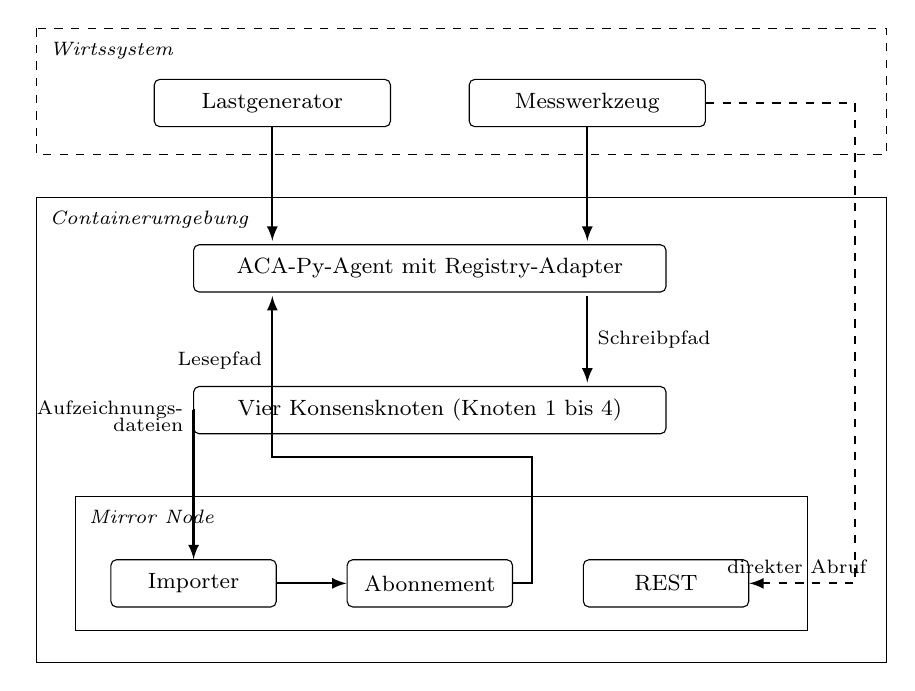
\begin{tikzpicture}[
      font=\footnotesize,
      box/.style={draw, rounded corners=2pt, minimum height=0.6cm, align=center},
      pfeil/.style={-latex, thick}
    ]
      \draw[dashed] (-5.4,0.85) rectangle (5.4,-0.75);
      \node[anchor=north west, font=\scriptsize\itshape] at (-5.35,0.8) {Wirtssystem};
      \node[box, minimum width=3.0cm] (last) at (-2.4,-0.1) {Lastgenerator};
      \node[box, minimum width=3.0cm] (mess) at (1.6,-0.1) {Messwerkzeug};

      \draw (-5.4,-1.3) rectangle (5.4,-7.2);
      \node[anchor=north west, font=\scriptsize\itshape] at (-5.35,-1.35) {Containerumgebung};
      \node[box, minimum width=6.0cm] (agent) at (-0.4,-2.2) {ACA-Py-Agent mit Registry-Adapter};
      \node[box, minimum width=6.0cm] (knoten) at (-0.4,-4.0) {Vier Konsensknoten (Knoten 1 bis 4)};
      \draw (-4.9,-5.1) rectangle (4.4,-6.8);
      \node[anchor=north west, font=\scriptsize\itshape] at (-4.85,-5.15) {Mirror Node};
      \node[box, minimum width=2.1cm] (imp) at (-3.4,-6.2) {Importer};
      \node[box, minimum width=2.1cm] (grpc) at (-0.4,-6.2) {Abonnement};
      \node[box, minimum width=2.1cm] (rest) at (2.6,-6.2) {REST};

      \draw[pfeil] (last) -- (-2.4,-1.85);
      \draw[pfeil] (mess) -- (1.6,-1.85);
      \draw[pfeil] (1.6,-2.55) -- node[right, font=\scriptsize] {Schreibpfad} (1.6,-3.65);
      \draw[pfeil] (knoten.west) -| node[left, pos=0.3, font=\scriptsize] {Aufzeichnungs-} node[left, pos=0.55, font=\scriptsize] {dateien} (imp.north);
      \draw[pfeil] (imp) -- (grpc);
      \draw[pfeil] (grpc.east) -- (0.9,-6.2) -- (0.9,-4.6) -- (-2.4,-4.6) -- node[left, pos=0.6, font=\scriptsize] {Lesepfad} (-2.4,-2.55);
      \draw[pfeil, dashed] (mess.east) -- (5.0,-0.1) -- (5.0,-6.2) -- node[above, pos=0.55, font=\scriptsize] {direkter Abruf} (rest.east);
    \end{tikzpicture}
    \caption{Verteilung der Komponenten der HCS-Variante auf Wirtssystem und Containerumgebung. Wesentlich für die Messung sind die beiden getrennten Lesepfade: Der Registry-Adapter liest über die Abonnementschnittstelle, ein direkter Abruf über die REST-Schnittstelle. Beide werden von unterschiedlichen Diensten bedient und dürfen nicht zu einer Lesedauer zusammengefasst werden (Abschnitt~\ref{subsec:impl-messpunkte}).}
    \label{fig:impl-deployment}
\end{figure}


\subsection{Anpassung des DID-SDK}
\label{subsec:impl-hcs-patch}

Die von der Erweiterung verwendete Bibliothek zur Auflösung und Registrierung von \texttt{did:hedera}-Bezeichnern~\cite{hierodidsdk} prüft die im Bezeichner enthaltene Netzwerkkennung gegen eine feste Liste zulässiger Werte. Diese Liste enthält die öffentlichen Hedera-Netzwerke, nicht jedoch die Kennung des lokal betriebenen Netzwerks. Da Entscheidung E1 ein selbst betriebenes Netzwerk vorschreibt, ist die Bibliothek in unveränderter Form für den Messaufbau nicht verwendbar.

Die vorgenommene Anpassung umfasst netto drei hinzugefügte Zeilen ohne Entfernungen, verteilt auf zwei Dateien und drei Fundstellen: die Aufnahme der Kennung in die Liste zulässiger Werte, deren Einbindung in der zweiten Datei und ihre Berücksichtigung in der Prüfkette. Die Semantik der Bibliothek wird dabei nicht verändert: Weder das Format des Bezeichners noch die Reihenfolge oder der Inhalt der abgesetzten Topic-Operationen noch das Nachrichtenformat sind berührt; dies wurde gegen den Patch im Einzelnen geprüft. Die Anpassung liegt damit vollständig auf der Validierungsebene und nicht auf dem gemessenen Pfad, was für die Aussagekraft der Messung wesentlich ist.

Bemerkenswert ist das Verhalten der unveränderten Bibliothek an dieser Stelle: Die Validierung erfolgt erst, nachdem die Registrierungsfunktion bereits ein Topic auf dem Netzwerk angelegt hat. Ein Registrierungsversuch mit einer nicht anerkannten Netzwerkkennung scheitert also nicht wirkungslos, sondern hinterlässt ein verwaistes Topic, das keiner DID zugeordnet ist und nicht mehr entfernt werden kann. Für den Aufbau bedeutet dies, dass fehlgeschlagene Registrierungsversuche vor Anwendung der Anpassung den Zustand des Netzwerks verändert haben; die Messungen wurden deshalb ausschließlich auf danach neu aufgebauten Netzwerken durchgeführt.

\begin{lstlisting}[basicstyle=\ttfamily\footnotesize, frame=single, caption={Fundstellen und Umfang der Anpassung}, label={lst:sdk-patch}]
Form:    Patchdatei, beim Bau des Abbilds angewandt
Umfang:  3 Zeilen hinzugefuegt, 0 entfernt (netto +3)
Stellen: 2 Dateien, 3 Fundstellen
         (1) Liste zulaessiger Netzkennungen: Kennung ergaenzt
         (2) Einbindung dieser Liste in der Validierungsdatei
         (3) Beruecksichtigung der Kennung in der Pruefkette
Wirkung: Kennung des lokalen Netzwerks wird als zulaessig anerkannt
Nicht beruehrt: Bezeichnerformat, Topic-Operationen, Nachrichtenformat
\end{lstlisting}


\section{Umsetzung der Indy-basierten Referenzvariante}
\label{sec:impl-indy}

Die Referenzvariante bildet die Ledger-Schicht der Referenzarchitektur nach~\cite{erler2023} und erfordert deutlich weniger Eigenleistung, da sie den in ACA-Py bereits enthaltenen Registry-Pfad verwendet. Betrieben wird ein lokales Indy-Netzwerk mit vier Validatorknoten, das über eine Genesis-Datei angebunden wird; die Knotenanzahl entspricht damit derjenigen der HCS-Variante, wie es NFA6 verlangt.

Eine Eigenschaft des Aufbaus ist für den späteren Vergleich zentral und wird deshalb hier und nicht erst in der Auswertung festgehalten. Bevor auf der Indy-Variante eine einzige Schema-Operation ausgeführt werden kann, muss die schreibende DID über eine NYM-Transaktion mit hinreichender Rolle auf dem Ledger registriert werden~\cite{torongo2023}. Ohne diesen Schritt wird der Schreibvorgang vom Ledger abgewiesen. Auf der HCS-Variante existiert zu diesem Schritt kein Gegenstück: Die schreibende DID entsteht zur Laufzeit, und die Topics der Identitätsobjekte sind nach E6 offen beschreibbar; die in E6 zusätzlich vorgesehene Vertrauenshierarchie wurde nicht umgesetzt (Abschnitt~\ref{sec:impl-befunde}, Befund B4). Der Aufbau der beiden Varianten unterscheidet sich damit nicht nur in der verwendeten Technologie, sondern in der Frage, ob überhaupt ein Berechtigungszustand hergestellt werden muss. Diese Asymmetrie ist kein Artefakt der Umsetzung, sondern der in Abschnitt~\ref{subsec:grundproblem-state-vs-ordering} beschriebene Unterschied zwischen einem zustandsführenden Ledger und einem reinen Ordnungsdienst in seiner unmittelbarsten Form; sie ist zugleich der Gegenstand des Szenarios S5 und wird in Abschnitt~\ref{sec:impl-befunde} als Befund geführt.

\subsection{Netzwerk, Abbildungsstand und Anbindung}
\label{subsec:impl-indy-netzwerk}

Das Indy-Netzwerk wird aus einem lokal erzeugten Container-Abbild betrieben, dessen Basis das im Ökosystem verbreitete Entwicklungsabbild für Indy-Knoten ist. Für die Reproduzierbarkeit ist an dieser Stelle eine Einschränkung festzuhalten, die beim Aufbau nicht beabsichtigt war und erst bei der Nachprüfung des Stands zutage trat: Der Versionsstand der Knoten ist ausschließlich über ein Abbild-Kennzeichen festgelegt und nicht über einen unveränderlichen Verweis. Ein solches Kennzeichen kann von seinem Herausgeber jederzeit auf einen anderen Abbildstand umgehängt werden; ein späterer Nachbau anhand derselben Angabe erzeugt daher nicht mit Sicherheit dasselbe Abbild. Weder ein Prüfwert des Abbilds noch ein Commit-Stand der zugrundeliegenden Quellen ist im Messaufbau festgehalten.

Für den Vergleich selbst ist dies ohne Folge, da alle Messungen beider Varianten gegen denselben, einmal erzeugten Abbildstand ausgeführt wurden. Für eine spätere Wiederholung der Messungen ist es dagegen eine echte Einschränkung, die in Abschnitt~\ref{sec:impl-grenzen} als Gültigkeitsgrenze geführt wird. Sie wäre durch das Festhalten des Abbild-Prüfwerts zu beheben gewesen und ist damit ein vermeidbarer Mangel der eigenen Vorgehensweise, kein Merkmal der verglichenen Technologien.

\begin{table}[htbp]
\renewcommand{\arraystretch}{1.3}
\footnotesize
  \centering
  \caption{Festgelegter Stand der Indy-Variante}
  \label{tab:impl-indy-stand}
  \begin{tabular}{p{0.30\textwidth} p{0.60\textwidth}}
    \toprule
    \textbf{Bestandteil} & \textbf{Festlegung} \\
    \midrule
    Knotenabbild & lokal erzeugt, ohne Versionskennzeichen \\
    Basisabbild & Entwicklungsabbild für Indy-Knoten, Kennzeichen \texttt{node-1.12-6}; veränderliches Kennzeichen, kein Prüfwert festgehalten \\
    Ledger-Bibliothek des Agenten & \texttt{indy-vdr} 0.4.2 \\
    Anbindung des Agenten & Genesis-Datei, in den Agenten-Container eingehängt \\
    Knotenanzahl & vier Validatorknoten \\
    \bottomrule
  \end{tabular}
\end{table}
\normalsize

Die Anbindung des Agenten erfolgt über die Genesis-Datei des Netzwerks, die dem Agenten-Container über eine Umgebungsvariable als Pfad bekannt gemacht und als Datei eingehängt wird. Sie wird nicht aus dem Netz bezogen, sondern liegt als Teil des Aufbaus vor, sodass der Agent auch ohne erreichbare Registrierungsdienste startet.

\subsection{Schreibberechtigung und ihre tatsächliche Durchsetzung}
\label{subsec:impl-indy-berechtigung}

Die schreibende DID des Agenten wird nicht zur Laufzeit erzeugt, sondern aus einem beim Start übergebenen Startwert abgeleitet. Verwendet wird dabei der öffentlich dokumentierte Entwicklungs-Startwert der eingesetzten Netzwerkdistribution, dem beim erstmaligen Hochfahren des Netzwerks die höchste Schreibrolle zugeordnet wird. Dieser Vorgang ist Bestandteil des Netzwerkstarts und nicht des Messaufbaus; die dabei entstehende Zuordnungsdatei liegt deshalb nicht im Messaufbau vor, sondern entsteht bei jedem Neuaufbau erneut. Der Nachweis der Rolle stützt sich damit auf das beobachtete Verhalten des Ledgers -- Schreibvorgänge werden angenommen, und die Rollenabfrage liefert den erwarteten Wert -- und nicht auf eine im Aufbau hinterlegte Konfigurationsangabe. Dass ein öffentlich bekannter Startwert verwendet wird, ist für einen Messaufbau unproblematisch und zugleich ein weiterer Beleg dafür, dass hier eine Entwicklungs- und keine Produktivkonfiguration betrieben wird (Abschnitt~\ref{sec:impl-grenzen}).

Beim Aufbau zeigte sich darüber hinaus, dass die ledgerseitige Rollenprüfung auf dem Weg über die Verwaltungsschnittstelle des Agenten nicht in der erwarteten Weise durchgreift: Der Agent signiert jede Ledger-Transaktion mit dieser seiner eigenen DID, unabhängig davon, welcher Aussteller im Rumpf der Anfrage angegeben ist. Da diese DID die höchste Schreibrolle besitzt, kann über die Verwaltungsschnittstelle auch im Namen einer Aussteller-DID geschrieben werden, die selbst keine Rolle besitzt.

Für den Messaufbau ist dies ohne Folge, da beide Varianten dieselbe Schnittstelle in derselben Weise nutzen und die Messgrößen davon unberührt bleiben. Für die Bewertung der Zugriffskontrolle ist es dagegen wesentlich und wird in Abschnitt~\ref{sec:impl-befunde} als eigenständiger Befund geführt: Die im Szenario S5 nachgewiesene rollenbasierte Schreibkontrolle ist eine Eigenschaft des Ledgers, nicht des Zugriffswegs, über den im Betrieb tatsächlich geschrieben wird. Aus diesem Grund werden die Prüfungen des Szenarios S5 nicht über die Verwaltungsschnittstelle, sondern über direkte Ledger-Aufrufe unterhalb des Agenten geführt (Abschnitt~\ref{subsec:impl-szenario-s5}).

% TODO Startparameter beider Varianten als Listing oder Tabelle ergaenzen: die vollstaendige Gegenueberstellung der Agenten-Startparameter je Variante samt Differenzliste liegt im Auditbericht des Messrepositoriums vor und ist von dort zu uebernehmen. Sie belegt oder widerlegt die im Text getroffene Aussage, die Agentenschicht sei in beiden Varianten identisch konfiguriert -- diese Aussage ist bis zur Uebernahme nicht belegt. Den Trustee-Startwert dabei NICHT abdrucken.


\section{Symmetrie und Abweichungen zwischen den Varianten}
\label{sec:impl-symmetrie}

Die zentrale methodische Voraussetzung des gesamten Vergleichs ist, dass die Messgrenze in beiden Varianten an derselben Stelle liegt (Abschnitt~\ref{subsec:eval-aufbau}). Diese Voraussetzung wird nicht behauptet, sondern am laufenden System geprüft. Als Prüfgröße dient die Menge der vom Agenten registrierten HTTP-Routen, da sie unmittelbar abbildet, welche Operationen über die Schnittstelle überhaupt erreichbar sind. Verglichen werden die Routenmengen beider Messvarianten sowie, als Kontrollfall, diejenige eines Agenten mit dem älteren Wallet-Typ.

\begin{table}[htbp]
\renewcommand{\arraystretch}{1.3}
\footnotesize
  \centering
  \caption{Vergleich der registrierten Routen beider Varianten und des Kontrollfalls}
  \label{tab:impl-routen}
  \begin{tabular}{p{0.30\textwidth} p{0.14\textwidth} p{0.42\textwidth}}
    \toprule
    \textbf{Konfiguration} & \textbf{Routen} & \textbf{Befund} \\
    \midrule
    HCS-Variante, \texttt{askar-anoncreds} & 169 & 23 Arbeitsrouten unter \texttt{/anoncreds/*} vorhanden \\
    Indy-Variante, \texttt{askar-anoncreds} & 168 & dieselben 23 Arbeitsrouten, identisch \\
    Kontrollfall, \texttt{askar} & 172 & keine \texttt{/anoncreds/*}-Arbeitsrouten; stattdessen 26 abweichende Routen \\
    \bottomrule
  \end{tabular}
\end{table}
\normalsize

Der Vergleich der beiden Messvarianten ergibt eine Differenz von genau einer Route, nämlich dem von der Hedera-Erweiterung zusätzlich bereitgestellten Registrierungsendpunkt für DIDs. Alle 23 Arbeitsrouten unter \texttt{/anoncreds/*}, über die die Evaluation ihre Last erzeugt, sind in beiden Varianten identisch vorhanden. Damit ist die symmetrische Lage der Messgrenze nicht nur konzeptionell begründet, sondern am laufenden System belegt. Der Kontrollfall zeigt zugleich, dass diese Symmetrie an den Wallet-Typ gebunden ist und nicht unabhängig davon besteht.

Neben dieser Übereinstimmung besteht eine Abweichung, die hier offen benannt wird. Die Installation der Hedera-Erweiterung stuft eine kryptografische Basisbibliothek gegenüber dem Basisabbild und der Indy-Variante um eine Patch-Version zurück; die Gesamtzahl installierter Pakete unterscheidet sich entsprechend zwischen den beiden Varianten. Die Rückstufung ist eine Folge der von der Erweiterung deklarierten Abhängigkeiten und lässt sich nicht auflösen, ohne die in Abschnitt~\ref{subsec:impl-hcs-komponenten} begründete Versionsfestlegung aufzugeben. Ein Einfluss auf die gemessenen Größen ist nicht zu erwarten, da die Bibliothek auf beiden Varianten nicht auf dem gemessenen Pfad liegt; ausgeschlossen werden kann er jedoch nicht, weshalb die Abweichung in Abschnitt~\ref{sec:impl-grenzen} als Gültigkeitsgrenze geführt wird.

\paragraph{Symmetriebedingung für den Widerruf.} Abschnitt~\ref{subsec:eval-validitaet} macht die messende Bewertung des Widerrufs davon abhängig, dass beide Varianten auf demselben Stand betrieben werden, da ein allein auf der HCS-Variante erhobener Wert kein Vergleich wäre. Diese Bedingung ist hier genauer zu fassen, als es die bloße Nennung des Wallet-Typs leisten würde.

Zu unterscheiden sind zwei Ebenen. Die Austausch-Protokolle für Ausstellung und Präsentation liegen in der Agentenschicht und damit außerhalb der Messgrenze (Abschnitt~\ref{sec:impl-ueberblick}); sie werden von der Evaluation nicht ausgeführt und sind für die Vergleichbarkeit der hier erhobenen Werte ohne Bedeutung. Was verglichen wird, ist ausschließlich das Objektmodell des Widerrufs auf der Ledger-Schicht: Widerrufsregister, Akkumulator und dessen Fortschreibung. Die Symmetriebedingung ist deshalb auf dieser Ebene einzulösen, und dort ist sie einlösbar: Beide Varianten werden mit dem Wallet-Typ \texttt{askar-anoncreds} und derselben AnonCreds-Bibliothek in derselben Version betrieben (Tabelle~\ref{tab:impl-versionsstand}), sodass Aufbau und Fortschreibung des Akkumulators auf beiden Varianten von derselben Implementierung ausgeführt werden. Unterschiedlich ist allein, auf welchem Ledger die entstehenden Objekte abgelegt werden -- und genau das ist der Gegenstand des Vergleichs.

Der vollständige Widerrufspfad -- Registrierung einer widerrufsfähigen Credential Definition, Anlage des Widerrufsregisters, initialer Eintrag, Fortschreibung des Akkumulators bei einem Widerruf und dessen Rücklesung -- wurde auf beiden Varianten unabhängig voneinander erfolgreich durchgeführt (Kapitel~\ref{sec:results}). Dabei ist eine Einschränkung des Wegs festzuhalten: Die Ausstellerlogik des Agenten verweigert die Anlage einer widerrufsfähigen Credential Definition ohne konfigurierten Tails-Dienst, obwohl der Ledger-Pfad selbst keinen solchen Dienst benötigt, um die Fortschreibung des Akkumulators zu beobachten. Der Widerrufspfad wurde deshalb auf beiden Varianten unterhalb des Agenten über direkte Aufrufe der jeweiligen Registry- beziehungsweise Ledger-Schnittstelle ausgeführt (Abschnitt~\ref{subsec:impl-szenario-s5}). Diese Umgehung ist in beiden Varianten gleichartig und berührt die Symmetrie daher nicht; sie bedeutet jedoch, dass der berichtete Widerrufspfad der Ledger-Pfad ist und nicht der Weg, den eine Ausstelleranwendung im Betrieb nehmen würde.


\section{Messmethodik}
\label{sec:impl-messmethodik}

\subsection{Messpunkte und Zeitnahme}
\label{subsec:impl-messpunkte}

Erhoben werden Zeitstempel an der Registry-Schnittstelle sowie Ressourcenmetriken aller Komponenten innerhalb der Messgrenze (Abschnitt~\ref{subsec:eval-aufbau}). Für die Latenzmessung nach NFA2 sind dabei drei Messpunkte zu unterscheiden, die auf der HCS-Variante nicht zusammenfallen.

\begin{table}[htbp]
\renewcommand{\arraystretch}{1.3}
\footnotesize
  \centering
  \caption{Messpunkte der Latenzmessung}
  \label{tab:impl-messpunkte}
  \begin{tabular}{p{0.20\textwidth} p{0.44\textwidth} p{0.22\textwidth}}
    \toprule
    \textbf{Messpunkt} & \textbf{Definition} & \textbf{Uhr} \\
    \midrule
    Schreibabschluss & Rückkehr des Aufrufs an der Registry-Schnittstelle & lokal \\
    Konsens & Konsens-Zeitstempel der Nachricht & Netzwerk \\
    Abrufbarkeit & Erster erfolgreicher Abruf des Objekts über die Mirror Node & lokal \\
    \bottomrule
  \end{tabular}
\end{table}
\normalsize

Auf der Indy-Variante fallen Schreibabschluss und Abrufbarkeit zusammen, da der Ledger den abgeleiteten Zustand unmittelbar mit dem Schreibvorgang fortschreibt (Abschnitt~\ref{subsec:grundlagen-speicher-indy}). Auf der HCS-Variante liegen sie auseinander; der Abstand zwischen ihnen ist keine eigenständige Vergleichsgröße, sondern eine Korrekturgröße, ohne deren Erfassung jeder HCS-Lesewert diesen Abstand unerkannt enthält und das Szenario S3 ungleiche Sachverhalte vergleichen würde.

Für den lesenden Zugriff ist zusätzlich zwischen zwei Pfaden zu unterscheiden, die in Abschnitt~\ref{subsec:impl-hcs-netzwerk} bereits als getrennte Dienste ausgewiesen wurden: dem Lesepfad des Registry-Adapters über die Abonnementschnittstelle und dem direkten Abruf über die REST-Schnittstelle. Beide werden getrennt erhoben und getrennt berichtet. Ihre Zusammenfassung zu einer einzigen Lesedauer wäre unzulässig, da sie unterschiedliche Dienste mit unterschiedlichem Verhalten messen; der Unterschied zwischen ihnen ist selbst ein Ergebnis und wird in Kapitel~\ref{sec:results} berichtet.

\begin{figure}[H]
    \centering
    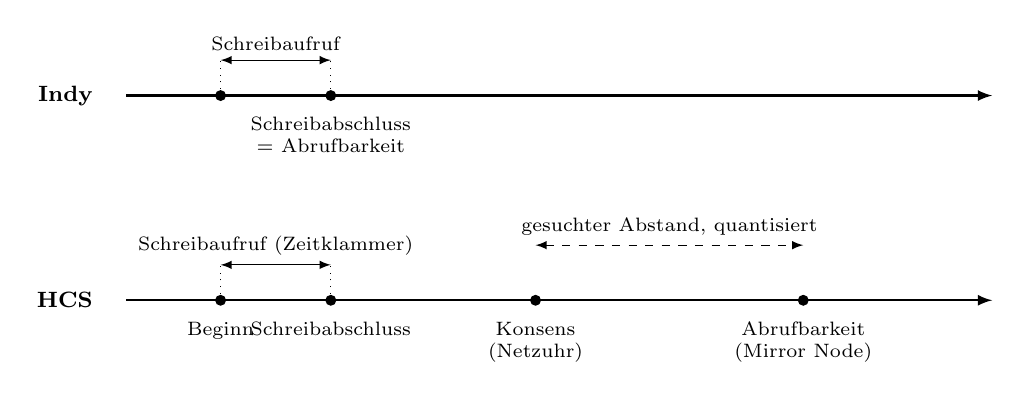
\begin{tikzpicture}[
      font=\footnotesize,
      marke/.style={circle, fill=black, inner sep=1.4pt},
      achse/.style={-latex, thick}
    ]
      \node[anchor=east, font=\footnotesize\bfseries] at (-0.3,0) {Indy};
      \draw[achse] (0,0) -- (11,0);
      \node[marke] (i1) at (1.2,0) {};
      \node[marke] (i2) at (2.6,0) {};
      \draw[latex-latex] (1.2,0.45) -- node[above, font=\scriptsize] {Schreibaufruf} (2.6,0.45);
      \draw[dotted] (1.2,0) -- (1.2,0.45);
      \draw[dotted] (2.6,0) -- (2.6,0.45);
      \node[anchor=north, align=center, font=\scriptsize] at (2.6,-0.15) {Schreibabschluss\\ = Abrufbarkeit};

      \node[anchor=east, font=\footnotesize\bfseries] at (-0.3,-2.6) {HCS};
      \draw[achse] (0,-2.6) -- (11,-2.6);
      \node[marke] (h1) at (1.2,-2.6) {};
      \node[marke] (h2) at (2.6,-2.6) {};
      \node[marke] (h3) at (5.2,-2.6) {};
      \node[marke] (h4) at (8.6,-2.6) {};
      \draw[latex-latex] (1.2,-2.15) -- node[above, font=\scriptsize] {Schreibaufruf (Zeitklammer)} (2.6,-2.15);
      \draw[dotted] (1.2,-2.6) -- (1.2,-2.15);
      \draw[dotted] (2.6,-2.6) -- (2.6,-2.15);
      \node[anchor=north, font=\scriptsize] at (1.2,-2.75) {Beginn};
      \node[anchor=north, font=\scriptsize] at (2.6,-2.75) {Schreibabschluss};
      \node[anchor=north, align=center, font=\scriptsize] at (5.2,-2.75) {Konsens\\ (Netzuhr)};
      \node[anchor=north, align=center, font=\scriptsize] at (8.6,-2.75) {Abrufbarkeit\\ (Mirror Node)};
      \draw[latex-latex, dashed] (5.2,-1.9) -- node[above, font=\scriptsize] {gesuchter Abstand, quantisiert} (8.6,-1.9);
    \end{tikzpicture}
    \caption{Messpunkte einer Schreib-Lese-Folge auf beiden Varianten. Auf der Indy-Variante fallen Schreibabschluss und Abrufbarkeit zusammen, auf der HCS-Variante nicht. Der Konsens-Zeitstempel stammt von einer anderen Uhr als die übrigen Marken, weshalb der Abstand zwischen Konsens und Abrufbarkeit nicht durch Differenzbildung, sondern über die Zeitklammer bestimmt wird (Abschnitt~\ref{subsec:impl-zeitklammer}).}
    \label{fig:impl-messpunkte}
\end{figure}


\subsection{Zwei-Uhren-Problem und Zeitklammer}
\label{subsec:impl-zeitklammer}

Der Abstand zwischen Konsens und Abrufbarkeit lässt sich nicht durch direkte Differenzbildung bestimmen. Der Konsens-Zeitstempel stammt von der Uhr des Netzwerks, der Zeitpunkt des ersten erfolgreichen Abrufs von der lokalen Uhr des Messrechners; die Differenz beider Werte vermischt die gesuchte Verzögerung mit einem unbekannten Uhrenversatz. Eine Synchronisation beider Uhren würde diesen Versatz nicht beseitigen, sondern nur verkleinern, und ihre Güte wäre selbst nicht überprüfbar.

Verwendet wird deshalb ein Verfahren, das ohne Vergleich zweier Uhren auskommt. Der Schreibaufruf wird auf der lokalen Uhr geklammert, indem unmittelbar vor und unmittelbar nach dem Aufruf ein Zeitstempel genommen wird. Der Konsens fällt notwendigerweise zwischen diese beiden Marken, da die Antwort des Aufrufs erst nach abgeschlossenem Schreibvorgang zurückkehrt. Aus der Klammer ergeben sich damit eine obere und eine untere Schranke des gesuchten Abstands, beide aus Differenzen derselben lokalen Uhr gebildet. Berichtet wird nicht ein Punktwert, sondern das Intervall.

Zwei Bedingungen sind für die Gültigkeit dieses Verfahrens einzuhalten. Erstens muss die Prämisse, dass der Konsens innerhalb der Klammer liegt, geprüft und nicht nur angenommen werden; sie wurde im Verlauf der Messungen mehrfach bestätigt. Zweitens muss die Abfrage auf Abrufbarkeit bereits im schreibenden Ablauf beginnen und nicht erst in einem nachgelagerten Schritt. Beginnt sie später, so ist das Objekt beim ersten Abfrageversuch bereits sichtbar, der Übergang von Nichtsichtbarkeit zu Sichtbarkeit wird nicht beobachtet, und es entsteht keine Klammer, sondern lediglich eine Obergrenze. Dieser Fall wird nicht stillschweigend als gültige Messung geführt, sondern durch eine im Messergebnis mitgeführte Markierung ausdrücklich als Obergrenze gekennzeichnet.

\begin{figure}[H]
    \centering
    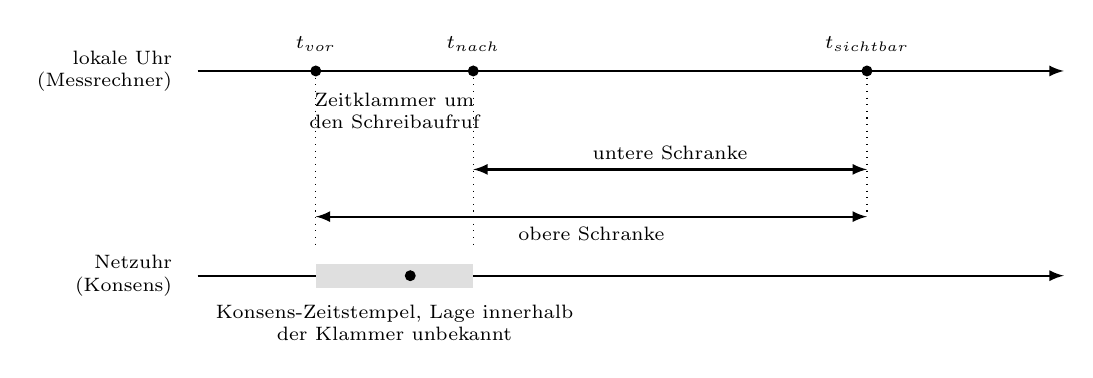
\begin{tikzpicture}[
      font=\footnotesize,
      marke/.style={circle, fill=black, inner sep=1.4pt},
      achse/.style={-latex, thick}
    ]
      \node[anchor=east, align=right, font=\scriptsize] at (-0.2,0) {lokale Uhr\\ (Messrechner)};
      \draw[achse] (0,0) -- (11,0);
      \node[marke] at (1.5,0) {};
      \node[marke] at (3.5,0) {};
      \node[marke] at (8.5,0) {};
      \node[anchor=south, font=\scriptsize] at (1.5,0.12) {$t_{\text{vor}}$};
      \node[anchor=south, font=\scriptsize] at (3.5,0.12) {$t_{\text{nach}}$};
      \node[anchor=south, font=\scriptsize] at (8.5,0.12) {$t_{\text{sichtbar}}$};
      \node[anchor=north, align=center, font=\scriptsize] at (2.5,-0.15) {Zeitklammer um\\ den Schreibaufruf};
      \draw[dotted] (1.5,0) -- (1.5,-2.2);
      \draw[dotted] (3.5,0) -- (3.5,-2.2);

      \node[anchor=east, align=right, font=\scriptsize] at (-0.2,-2.6) {Netzuhr\\ (Konsens)};
      \draw[achse] (0,-2.6) -- (11,-2.6);
      \fill[gray!25] (1.5,-2.75) rectangle (3.5,-2.45);
      \node[marke] at (2.7,-2.6) {};
      \node[anchor=north, align=center, font=\scriptsize] at (2.5,-2.85) {Konsens-Zeitstempel, Lage innerhalb\\ der Klammer unbekannt};

      \draw[latex-latex, thick] (3.5,-1.25) -- node[above, font=\scriptsize] {untere Schranke} (8.5,-1.25);
      \draw[latex-latex, thick] (1.5,-1.85) -- node[below, font=\scriptsize] {obere Schranke} (8.5,-1.85);
      \draw[dotted] (8.5,0) -- (8.5,-1.85);
    \end{tikzpicture}
    \caption{Zeitklammer um den Schreibaufruf. Der Konsens liegt notwendigerweise zwischen $t_{\text{vor}}$ und $t_{\text{nach}}$, seine genaue Lage innerhalb dieses Fensters ist jedoch nicht bestimmbar (grau). Obere und untere Schranke des Abstands zwischen Konsens und Abrufbarkeit werden ausschließlich aus Differenzen der lokalen Uhr gebildet; ein Uhrenvergleich findet nicht statt. Berichtet wird das Intervall, nicht ein Punktwert.}
    \label{fig:impl-zeitklammer}
\end{figure}


\subsection{Quantisierung der Sichtbarkeit und Phasenzerlegung}
\label{subsec:impl-phasenzerlegung}

Der so bestimmte Abstand ist keine kontinuierliche Größe. Die Mirror Node übernimmt Nachrichten nicht einzeln, sondern in geschlossenen Aufzeichnungsdateien; die Sichtbarkeit eines Objekts springt daher erst mit dem Abschluss der Datei, in der es enthalten ist. Ein Einzelwert setzt sich damit aus zwei Anteilen zusammen: der verbleibenden Laufzeit der Aufzeichnungsdatei bis zu ihrem Abschluss, im Folgenden als Phasenanteil bezeichnet, und der eigentlichen Verarbeitungszeit der abgeschlossenen Datei. Nur der zweite Anteil ist eine Eigenschaft der Verarbeitungskette; der erste hängt allein davon ab, an welcher Stelle des laufenden Aufzeichnungsintervalls der Schreibvorgang einfällt, und ist damit eine Eigenschaft des Messzeitpunkts, nicht des Systems.

Der Phasenanteil ist rückwirkend bestimmbar, weil der Dateiname einer Aufzeichnungsdatei den Konsens-Zeitstempel ihrer ersten Transaktion trägt. Aus dem Protokoll des Importers lässt sich damit für jedes gemessene Objekt der Beginn der zugehörigen Datei rekonstruieren und der Phasenanteil aus dem Einzelwert herausrechnen. Jede Ingest-Messung wird deshalb in Phasenanteil und Verarbeitungsanteil zerlegt; berichtet und in den Vergleich eingesetzt wird der Verarbeitungsanteil, während der Phasenanteil als Eigenschaft des Betriebszustands getrennt ausgewiesen wird. Die Wirksamkeit dieser Zerlegung wurde an einer eigenen Messreihe geprüft; die Werte werden in Kapitel~\ref{sec:results} berichtet.

Für die Deutung des Phasenanteils ist eine Beobachtung wesentlich, die den zunächst naheliegenden Modellansatz korrigiert. Man würde erwarten, dass ein Schreibvorgang zu einem zufälligen Zeitpunkt in ein bereits laufendes Aufzeichnungsintervall fällt und der Phasenanteil entsprechend gleichverteilt zwischen null und der Intervalldauer liegt. Tatsächlich lag der Konsens-Zeitstempel bei nahezu allen gemessenen Objekten exakt am Beginn der zugehörigen Datei: Der Schreibvorgang eröffnet die Datei selbst. Der Phasenanteil entspricht damit der vollen Dauer des Intervalls und nicht einem zufälligen Anteil davon. Die aus der Zerlegung gezogenen Schlussfolgerungen bleiben davon unberührt, ihre Begründung ist jedoch eine andere.

Die Dauer des Aufzeichnungsintervalls ist ihrerseits keine Konstante, sondern hängt vom anliegenden Verkehr ab; sie ist auf einem stärker belasteten Netzwerk deutlich kürzer als auf einem leerlaufenden. Sie wird deshalb je Messpaar erfasst und nicht als globaler Parameter angenommen. Genau diese Verkehrsabhängigkeit ist zugleich die Begründung der im folgenden Abschnitt beschriebenen Grundlast.

\begin{figure}[H]
    \centering
    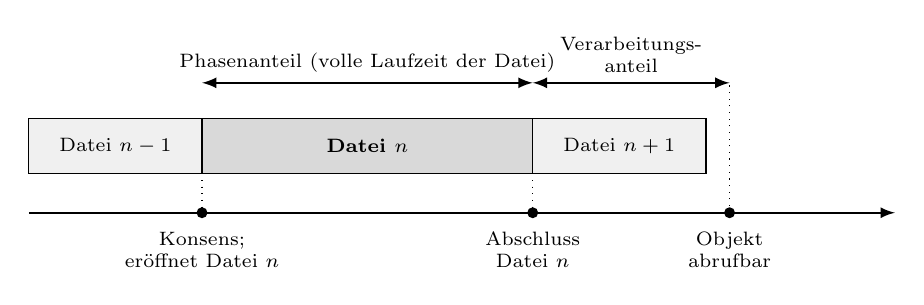
\begin{tikzpicture}[
      font=\footnotesize,
      marke/.style={circle, fill=black, inner sep=1.4pt},
      achse/.style={-latex, thick}
    ]
      \draw[fill=gray!12] (0,0) rectangle (2.2,0.7);
      \draw[fill=gray!30] (2.2,0) rectangle (6.4,0.7);
      \draw[fill=gray!12] (6.4,0) rectangle (8.6,0.7);
      \node[font=\scriptsize] at (1.1,0.35) {Datei $n-1$};
      \node[font=\scriptsize] at (4.3,0.35) {\textbf{Datei $n$}};
      \node[font=\scriptsize] at (7.5,0.35) {Datei $n+1$};
      \draw[achse] (0,-0.5) -- (11,-0.5);
      \node[marke] at (2.2,-0.5) {};
      \node[marke] at (6.4,-0.5) {};
      \node[marke] at (8.9,-0.5) {};
      \draw[dotted] (2.2,0) -- (2.2,-0.5);
      \draw[dotted] (6.4,0) -- (6.4,-0.5);
      \node[anchor=north, align=center, font=\scriptsize] at (2.2,-0.62) {Konsens;\\ eröffnet Datei $n$};
      \node[anchor=north, align=center, font=\scriptsize] at (6.4,-0.62) {Abschluss\\ Datei $n$};
      \node[anchor=north, align=center, font=\scriptsize] at (8.9,-0.62) {Objekt\\ abrufbar};
      \draw[latex-latex, thick] (2.2,1.15) -- node[above, font=\scriptsize] {Phasenanteil (volle Laufzeit der Datei)} (6.4,1.15);
      \draw[latex-latex, thick] (6.4,1.15) -- node[above, font=\scriptsize, align=center] {Verarbeitungs-\\anteil} (8.9,1.15);
      \draw[dotted] (8.9,-0.5) -- (8.9,1.15);
    \end{tikzpicture}
    \caption{Zerlegung des Abstands zwischen Konsens und Abrufbarkeit in Phasenanteil und Verarbeitungsanteil. Der Schreibvorgang eröffnet die Aufzeichnungsdatei selbst, der Phasenanteil entspricht deshalb deren voller Laufzeit und nicht einem zufälligen Anteil davon. Nur der Verarbeitungsanteil ist eine Eigenschaft der Verarbeitungskette und geht in den Vergleich ein; die Laufzeit der Datei hängt vom anliegenden Verkehr ab und wird je Messpaar erfasst.}
    \label{fig:impl-phasenzerlegung}
\end{figure}


\subsection{Grundlast}
\label{subsec:impl-grundlast}

Abschnitt~\ref{subsec:eval-szenarien} legt fest, dass alle Szenarien einschließlich der Basismessung S1 unter einer definierten und protokollierten Grundlast statt auf einem leerlaufenden Netzwerk ausgeführt werden. Dieser Abschnitt legt die Grundlast fest und begründet ihre Ausgestaltung.

Die Notwendigkeit ergibt sich aus dem im vorigen Abschnitt beschriebenen Mechanismus. Auf einem vollständig leerlaufenden Netzwerk bleibt die Aufzeichnungsdatei mangels weiteren Verkehrs offen und unsigniert; die Sichtbarkeit ist damit nicht zeitgetrieben, sondern verkehrsgetrieben. Ohne Grundlast würde die gemessene Lesedauer nicht die Verarbeitungskette abbilden, sondern den Umstand, dass nach dem Messobjekt keine weitere Nachricht mehr eintraf. Gemessen würde also eine Eigenschaft des Messaufbaus und nicht eine Eigenschaft der Technologie.

Umgesetzt wird die Grundlast als gleichmäßig getakteter Nachrichtenstrom auf einem eigenen, von den Messobjekten getrennten Topic. Das Taktintervall beträgt drei Sekunden und wird über die gesamte Dauer jeder Messung aufrechterhalten. Die Gebühren dieses Stroms werden bewusst nicht aus dem Konto beglichen, das die Messoperationen ausführt, sondern aus einem separaten Konto. Der Grund ist, dass die Kontostandsänderung des ausführenden Kontos selbst als Beleg für die Anzahl tatsächlich abgesetzter Nachrichten verwendet wird; eine Vermischung mit dem Grundlaststrom würde diesen Beleg unbrauchbar machen.

Der Betrieb der Grundlast wird während jeder Messung überwacht. Ein stillschweigender Abriss des Stroms führt nicht zu einem Fehler, sondern zu unauffällig zu hohen Messwerten und ist damit die gefährlichere Fehlerart; die Überwachung ist in Abschnitt~\ref{sec:impl-betrieb} beschrieben.


\subsection{Zwischenspeicher, Wiederholungen und Lasterzeugung}
\label{subsec:impl-wiederholungen}

Der Registry-Adapter hält aufgelöste Objekte in einem Zwischenspeicher mit einer Gültigkeitsdauer von einer Stunde vor. Für die Latenzmessung nach NFA2 ist dabei zweierlei festzuhalten. Erstens wird nur ein erfolgreicher Auflösungsvorgang abgelegt; ein fehlgeschlagener Versuch wird nicht abgelegt, da die Ablage im Programmablauf hinter der Rückkehr des Fehlerfalls liegt. Ein wiederholter Abruf eines noch nicht sichtbaren Objekts wird also tatsächlich erneut ausgeführt und nicht aus dem Zwischenspeicher beantwortet. Zweitens wird derselbe Zwischenspeicher von mehreren Objekttypen gemeinsam genutzt. Eine Messung des ungepufferten Lesewegs erfordert deshalb einen jeweils frisch angelegten Zwischenspeicher; andernfalls misst die zweite Leseoperation einer Messreihe nicht mehr den Ledger, sondern den Zwischenspeicher. Gemessen und berichtet werden beide Fälle getrennt, da der gepufferte Fall dem realen Betriebsverhalten und der ungepufferte dem Verhalten der Ledger-Schicht entspricht.

Die Lasterzeugung für die Szenarien S2 und S4 erfolgt über ein eigenständiges Lastwerkzeug~\cite{locust}, das außerhalb der Container auf dem Wirtssystem betrieben wird. Diese Anordnung stellt sicher, dass der Ressourcenverbrauch des Lastgenerators nicht in die nach NFA3 erhobenen Ressourcenmetriken der Komponenten innerhalb der Messgrenze eingeht.

\subsection{Wiederholungen, Warmlauf und Auswertungskennzahl}
\label{subsec:impl-kennzahl}

Abschnitt~\ref{subsec:eval-szenarien} lässt die Wiederholungsanzahl je Messpunkt offen; sie wird hier festgelegt. Für alle Messreihen der Basismessung gilt eine Serienlänge von fünfzehn auswertbaren Läufen je Variante und Messpunkt. Der Warmlauf wird nicht über eine Zeitdauer, sondern über einen eigenen Lauf geregelt: Der erste Lauf jeder Serie ist ein Funktionsnachweis, der die Erreichbarkeit aller Komponenten und die Vollständigkeit der erzeugten Felder prüft, und wird von der Auswertung ausgeschlossen. Dieser Ausschluss erfolgt nicht nachträglich anhand der Messwerte, sondern anhand der Laufnummer, und ist damit kein Aussortieren auffälliger Werte. Wo eine Serie aus anderen Gründen mehr Rohläufe enthält, wird die Auswahl im Auswertungsstand ausdrücklich vermerkt.

Die übrigen Szenarien folgen ihrer jeweiligen Struktur: Die Laststeigerung besteht aus aufeinanderfolgenden Stufen und wird nicht wiederholt, sondern bis zum Eintreten eines Abbruchkriteriums fortgesetzt; das Datenwachstum wird an festen Zwischenständen erhoben; der Knotenausfall wird je Variante fünfmal wiederholt; die Prüfungen der Zugriffskontrolle sind Einzelnachweise ohne Serie, da ihr Ergebnis nicht metrisch, sondern binär ist. Tabelle~\ref{tab:impl-wiederholungen} fasst dies zusammen.

\begin{table}[htbp]
\renewcommand{\arraystretch}{1.3}
\footnotesize
  \centering
  \caption{Wiederholungsanzahl und Auswertungsform je Szenario}
  \label{tab:impl-wiederholungen}
  \begin{tabular}{p{0.10\textwidth} p{0.40\textwidth} p{0.40\textwidth}}
    \toprule
    \textbf{Szenario} & \textbf{Wiederholungen} & \textbf{Auswertungsform} \\
    \midrule
    S1 & 15 auswertbare Läufe je Variante und Messpunkt, erster Lauf als Funktionsnachweis ausgeschlossen & Median mit robuster Streuung, Trendprüfung über die Laufreihenfolge \\
    S2 & keine Wiederholung; aufeinanderfolgende Laststufen bis zum Abbruchkriterium & Kennwerte je Stufe, Sättigungspunkt \\
    S3 & drei Lesungen des Zielobjekts je Zwischenstand, zusätzlich eine Kontrolllesung je Zwischenstand & Verlauf über die Bestandsgröße \\
    S4 & 5 Läufe je Variante & Median mit robuster Streuung über die Läufe \\
    S5 & Einzelnachweise ohne Serie & binäres Ergebnis mit Belegkette \\
    \bottomrule
  \end{tabular}
\end{table}
\normalsize

Als Kennzahl der Lage dient durchgehend der Median und als Streuungsmaß die skalierte mittlere absolute Abweichung. Das arithmetische Mittel und die Standardabweichung werden nicht verwendet, da die beobachteten Verteilungen schwere Ränder aufweisen und einzelne Ausreißer -- etwa ein einzelner Lauf mit abgerissenem Grundlaststrom -- die Standardabweichung dominieren würden, ohne dass sich das typische Verhalten geändert hätte. Aus demselben Grund wird für den Vergleich gepaarter Größen der Wilcoxon-Vorzeichen-Rang-Test und nicht der t-Test eingesetzt, und die Prüfung auf einen Trend über die Laufreihenfolge erfolgt über den Rangkorrelationskoeffizienten nach Spearman. Diese Trendprüfung ist nicht bloß eine Formalie: Sie hat im Verlauf der Arbeit eine kontaminierte Messreihe aufgedeckt, deren Werte über die Serie hinweg systematisch anstiegen, weil die jeweils andere Variante noch Arbeitsspeicher belegte; diese Serie wurde verworfen und unter der in Abschnitt~\ref{sec:impl-betrieb} beschriebenen Ein-Arm-Regel neu erhoben.

Die Bestandsgrößen für das Datenwachstum werden ebenfalls hier festgelegt und lösen den entsprechenden offenen Punkt aus Abschnitt~\ref{subsec:eval-szenarien} ein. Gemessen wird an vier Zwischenständen mit 10, 30, 100 und 300 zusätzlichen Füllobjekten, also über eine dreißigfache Spanne; die Staffelung ist ungefähr geometrisch gewählt, da ein etwaiger Effekt eher mit der Größenordnung als mit der absoluten Anzahl zu erwarten ist. Je Zwischenstand werden zwei Werte erhoben: die erneute Lesung desselben, unveränderten Zielobjekts und die Lesung eines nie zuvor gelesenen Füllobjekts. Die zweite Messung ist notwendig, weil ein flacher Verlauf des Zielobjekts allein auch dann entstünde, wenn der Lesepfad gar nicht mehr ausgeführt, sondern aus dem Zwischenspeicher bedient würde; erst ein ebenfalls flacher Verlauf der Kontrolllesung schließt diese Erklärung aus.

\subsection{Messwerkzeug}
\label{subsec:impl-werkzeug}

Die Messungen werden nicht über Ad-hoc-Aufrufe, sondern über ein eigens erstelltes Python-Paket ausgeführt. Der Anlass für diese Entscheidung ist selbst ein Messbefund: Die zuvor verwendeten Kommandozeilenskripte erzeugten für jeden einzelnen Zeitstempel einen eigenen Unterprozess, dessen Startkosten in der Größenordnung einiger zehn Millisekunden lagen und mehrfach je Abfragedurchlauf anfielen. Da die zu messenden Größen teilweise selbst im Bereich weniger Millisekunden liegen, verschob dieser Aufwand die Werte spürbar. Die mit den Skripten erhobenen Reihen liegen deshalb auf einer anderen Zeitbasis und werden nicht mit den späteren Werten vermischt; sie sind vollständig neu erhoben worden.

Das Paket ist nach Messaufgaben gegliedert: je ein Modul für den Schreibpfad beider Varianten, ein Modul für die Rücklesung, je ein Modul für die Szenarien der Laststeigerung, des Datenwachstums, des Knotenausfalls und der Zugriffskontrolle sowie ein gemeinsames Modul für die Serienführung. Letzteres vergibt die Laufnummern, schreibt jeden Lauf sowohl als Einzeldatei mit allen Rohfeldern als auch als Zeile in eine fortlaufende Serienübersicht und versieht beides mit dem in Abschnitt~\ref{sec:impl-betrieb} beschriebenen Aufbaustempel. Die Trennung beider Ausgabeformen ist bewusst: Die Serienübersicht führt nur eine festgelegte Auswahl von Feldern und eignet sich für den Überblick, nicht jedoch als alleinige Auswertungsgrundlage, da ein Lauf dort unauffällig erscheinen kann, dessen Einzeldatei eine sehr niedrige Erfolgsquote ausweist.

Das Paket ist durch eine automatisierte Testsuite abgedeckt, die 489 Testfälle umfasst und vollständig ohne laufendes Netzwerk ausführbar ist; kein Testfall setzt Netz-, Container- oder Ledger-Zugriff voraus. Im Abgabestand laufen alle 489 Testfälle fehlerfrei durch. Ihr Zweck ist nicht die Prüfung der Messwerte, die sie nicht erbringen kann, sondern die Prüfung der Messlogik: Zerlegung der Zeitwerte, Auswahl- und Abbruchkriterien, Feldbelegung und Serienführung. Die vollständige Ausführbarkeit ohne Messnetzwerk war dabei kein Nebenprodukt, sondern Voraussetzung der Arbeitsteilung: Sie erlaubte es, den überwiegenden Teil der Werkzeugentwicklung auf einem anderen Rechner durchzuführen und die knappe Zeit am Messaufbau ausschließlich für Messungen zu verwenden.

% TODO Optional als Anhang: Modulübersicht des Messwerkzeugs mit Dateinamen und Aufrufsyntax je Modul. Testfallzahl (489) und Bestehensstand sind geprueft und im Text eingetragen.


\section{Umsetzung der Evaluationsszenarien}
\label{sec:impl-szenarien}

Die Szenarien S1 bis S5 sind im Evaluationskonzept als Messaufgaben beschrieben. Dieser Abschnitt beschreibt, mit welchen Mitteln sie ausgeführt werden, und begründet dort, wo der naheliegende Weg nicht gangbar war, den gewählten Umweg.

\paragraph{S1 -- Basismessung.} Jeder Lauf führt die Schreiboperationen über die Registry-Schnittstelle des Agenten aus und klammert dabei jeden Aufruf einzeln (Abschnitt~\ref{subsec:impl-zeitklammer}). Die Lesewerte werden nicht im selben Lauf erhoben, sondern in einem eigenen Ablauf gegen die zuvor geschriebenen Objekte, damit der Lesepfad einen frisch angelegten Zwischenspeicher vorfindet (Abschnitt~\ref{subsec:impl-wiederholungen}). Die Werte des Widerrufspfads werden aus den in Abschnitt~\ref{subsec:impl-szenario-s5} beschriebenen Gründen nicht über die Ausstellerlogik des Agenten, sondern über direkte Ledger-Aufrufe erhoben; sie sind in vier getrennte Felder zerlegt -- Anlage des Registers, initialer Eintrag, eigentlicher Widerruf und Rücklesung des Akkumulatorzustands -- statt in einer einzigen Gesamtdauer zusammengefasst, da diese vier Schritte unterschiedliche Operationen sind und ihre Zusammenfassung die Herkunft der Dauer verdecken würde.

\paragraph{S2 -- Laststeigerung.} Die Last wird über das bereits für die Grundlast eingesetzte Lastwerkzeug erzeugt, hier jedoch mit schrittweise erhöhter Nebenläufigkeit statt mit festem Takt. Nach jeder Stufe werden drei Abbruchkriterien geprüft: ein Plateau des Durchsatzes, das Überschreiten eines Vielfachen der Ausgangsantwortzeit und das Überschreiten einer Fehlerratenschwelle. Die drei Kriterien sind gleichrangig und nicht hierarchisch angeordnet; welches zuerst greift, ist selbst ein Ergebnis. Diese Anordnung erwies sich als notwendig: Auf der HCS-Variante greift ausschließlich das Fehlerratenkriterium, während die Antwortzeit an der Sättigungsstelle sogar fällt, weil scheiternde Anfragen nahezu sofort beantwortet werden. Ein allein auf die Antwortzeit gestütztes Kriterium hätte die Sättigung dort nicht erkannt.

Die Ausgangsantwortzeit, gegen die das Vielfache gebildet wird, wird nicht aus der Basismessung des Schema-Schreibpfads übernommen, sondern aus dem im Leerlauf gemessenen Boden derselben Variante; sie beträgt 3010\,ms auf der Indy-Variante und 5070\,ms auf der HCS-Variante. Der ursprünglich verwendete Indy-Wert lag mit 1808\,ms unterhalb dieses Bodens und hätte das Kriterium bereits im unbelasteten Zustand ausgelöst.

\paragraph{S3 -- Datenwachstum.} Die Füllobjekte werden vor jedem Zwischenstand erzeugt, anschließend werden Zielobjekt und Kontrollobjekt gelesen. Auf der HCS-Variante musste der Ablauf nach einem ersten, verworfenen Durchlauf geändert werden: Der Registry-Adapter hält einen Zwischenspeicher, den sich mehrere Objekttypen teilen, sodass die Lesungen der späteren Zwischenstände nicht mehr den Ledger, sondern diesen Zwischenspeicher gemessen haben. Der Verlauf war dadurch flach, aber aus dem falschen Grund. Behoben wurde dies, indem der Agenten-Container vor den Lesungen jedes Zwischenstands neu erzeugt wird; der Zwischenspeicher ist danach leer. Der korrigierte Durchlauf zeigt denselben flachen Verlauf, nun jedoch mit tatsächlich ausgeführtem Lesepfad -- ein Beispiel dafür, dass ein unauffälliges Ergebnis erst dann aussagekräftig ist, wenn der Weg dorthin nachweislich beschritten wurde.

\paragraph{S4 -- Knotenausfall.} Der Ausfall wird auf beiden Varianten gezielt herbeigeführt, mit unterschiedlichen Mitteln: auf der Indy-Variante über das Anhalten des Containers des Zielknotens, auf der HCS-Variante über die Verwaltungsschnittstelle des Bereitstellungswerkzeugs, da ein Herunterskalieren der Container dort die Plattforminstallation zerstören würde (Abschnitt~\ref{sec:impl-betrieb}). Ein einzelner Knoten lässt sich über diese Schnittstelle nur mit einem Aufrufparameter ansprechen, der in der Werkzeugdokumentation für das Anhalten nicht ausgewiesen ist; seine Verwendbarkeit wurde am laufenden System nachgewiesen, bevor das Szenario ausgeführt wurde.

Zwei Eigenschaften dieses Aufbaus sind für die Deutung der Werte wesentlich und werden deshalb hier und nicht erst in der Auswertung festgehalten. Erstens beendet das Anhalten eines Containers den Prozess nicht sofort, sondern räumt ihm eine Frist zum geordneten Beenden ein; die Zeitspanne bis zum bestätigten Ende des Prozesses gehört nicht in die Ausfallphase, da das System in ihr noch arbeitet. Die Auswertung stützt sich deshalb auf den bestätigten Zeitpunkt des Prozessendes und nicht auf den Zeitpunkt des Anhaltebefehls. Zweitens benötigen die Verwaltungsbefehle des Bereitstellungswerkzeugs selbst jeweils eine bis zwei Minuten, da sie auf den vollständig wiederhergestellten Betriebszustand warten; ein erheblicher Anteil der auf der HCS-Variante gemessenen Ausfall- und Wiederherstellungsdauern ist damit Ausführungszeit des Werkzeugs und keine Eigenschaft des Netzwerks. Beide Punkte begrenzen die Vergleichbarkeit der absoluten Dauern zwischen den Varianten und werden in Abschnitt~\ref{sec:impl-grenzen} als Gültigkeitsgrenze geführt.

\paragraph{S5 -- Zugriffskontrolle und Widerruf.}
\label{subsec:impl-szenario-s5}
Die Prüfungen dieses Szenarios werden bewusst nicht über die Verwaltungsschnittstelle des Agenten geführt, sondern über direkte Aufrufe der darunterliegenden Ledger- beziehungsweise Registry-Schnittstelle. Dafür gibt es zwei voneinander unabhängige Gründe.

Der erste betrifft die Zugriffskontrolle selbst. Wie in Abschnitt~\ref{subsec:impl-indy-berechtigung} beschrieben, signiert der Agent jede Ledger-Transaktion mit seiner eigenen DID. Eine über die Verwaltungsschnittstelle ausgeführte Prüfung würde deshalb nicht die Berechtigung der geprüften DID messen, sondern stets diejenige des Agenten; sie könnte einen unberechtigten Schreibversuch gar nicht erzeugen. Erst unterhalb des Agenten lässt sich eine Transaktion mit einem gewählten Schlüssel signieren und damit die Regel des Ledgers tatsächlich prüfen.

Der zweite betrifft den Widerruf. Die Ausstellerlogik des Agenten verweigert die Anlage einer widerrufsfähigen Credential Definition, solange kein Tails-Dienst konfiguriert ist. Dieser Dienst wird für die Ausstellung von Nachweisen benötigt, nicht jedoch für die Beobachtung des Akkumulators auf dem Ledger. Da die Evaluation ausschließlich die Ledger-Schicht betrachtet, wäre der Aufbau eines Tails-Dienstes ein Aufwand außerhalb der Messgrenze gewesen, der am gemessenen Gegenstand nichts geändert hätte.

Die Umgehung ist auf beiden Varianten gleichartig aufgebaut und berührt die Symmetrie des Vergleichs daher nicht. Sie bedeutet jedoch, dass die Ergebnisse dieses Szenarios Aussagen über die Ledger-Schicht sind und nicht über den Weg, den eine Anwendung im Betrieb nehmen würde -- eine Unterscheidung, die für die Bewertung der Zugriffskontrolle wesentlich ist und in Kapitel~\ref{sec:discussion} aufgegriffen wird.

% TODO Kompakte Parametertabelle je Szenario-Modul ergaenzen (Aufrufsyntax, Stufenraster und Schwellwerte S2, Zielknoten und Beobachtungsfenster S4). Die vollstaendigen Tabellen mit Datei- und Zeilenangaben liegen im Auditbericht des Messrepositoriums vor; die im Text genannten Einzelwerte sind daraus bereits uebernommen.


\section{Betriebliche Randbedingungen und Reproduzierbarkeit}
\label{sec:impl-betrieb}

Der Messaufbau wird auf einem einzelnen Arbeitsplatzrechner betrieben. Die Tabelle~\ref{tab:impl-umgebung} weist die Ausführungsumgebung aus und löst damit die in Abschnitt~\ref{subsec:eval-aufbau} offen gelassene Festlegung ein.

\begin{table}[htbp]
\renewcommand{\arraystretch}{1.3}
\footnotesize
  \centering
  \caption{Ausführungsumgebung des Messaufbaus}
  \label{tab:impl-umgebung}
  \begin{tabular}{p{0.34\textwidth} p{0.56\textwidth}}
    \toprule
    \textbf{Merkmal} & \textbf{Wert} \\
    \midrule
    Prozessorarchitektur & x86-64 \\
    Arbeitsspeicher des Wirtssystems & 27,7 GB nutzbar \\
    Der Containerlaufzeit zugewiesen & 14 Prozessorkerne, 19,53 GiB Arbeitsspeicher \\
    Betriebssystem und Laufzeitumgebung & Windows mit Linux-Subsystem, containerisierte Ausführung \\
    \bottomrule
  \end{tabular}
\end{table}
\normalsize
% TODO Vier Werte am Messrechner ablesen und in die Tabelle eintragen: (1) genaue Prozessorbezeichnung und Grundtaktfrequenz, (2) Betriebssystemversion einschliesslich Build, (3) Version der Containerlaufzeit, (4) Version des Linux-Subsystems. Alle vier sind Angaben zum Messrechner und stehen in keiner Datei des Repositoriums; ohne sie bleibt die Ausfuehrungsumgebung nicht vollstaendig reproduzierbar beschrieben.

Aus dieser Umgebung ergibt sich die wichtigste betriebliche Regel des Aufbaus: Es wird immer nur eine der beiden Varianten betrieben, niemals beide gleichzeitig. Die Regel ist nicht vorsorglich gesetzt, sondern gemessen begründet. Der gleichzeitige Betrieb beider Varianten erschöpft den verfügbaren Arbeitsspeicher; der Abbau einer Variante gab 17,4 GB frei und hob den verfügbaren Speicher von 1,1 GB auf 17,4 GB, wobei die Systemlast um mehr als eine Größenordnung fiel und das anschließende Hochfahren der zweiten Variante innerhalb von 20 Sekunden statt in wiederholten Neustartversuchen abgeschlossen war. Unter Speicherdruck gemessene Werte wären keine Eigenschaften der Ledger-Technologien, sondern Eigenschaften der Konkurrenz beider Varianten um dieselben Ressourcen. Die Regel wird nicht durch Disziplin, sondern durch das Umschaltwerkzeug und durch eine Vorbedingungsprüfung in den Messskripten durchgesetzt, die bei Verletzung abbrechen.

Drei weitere Regeln betreffen die Unversehrtheit des Aufbaus über mehrere Messsitzungen hinweg. Erstens wird die Containerlaufzeit vor jedem Herunterfahren des Rechners geordnet beendet; ein abruptes Beenden zerreißt die Kontinuität der Aufzeichnungsdateien der Mirror Node irreparabel, was im Verlauf der Arbeit mehrfach eintrat und jeweils einen vollständigen Neuaufbau erforderte. Zweitens werden die Konsensknoten ausschließlich über die Verwaltungsschnittstelle des Bereitstellungswerkzeugs angehalten und gestartet, nie durch Herunterskalieren ihrer Container, da die Plattforminstallation nicht auf einem dauerhaften Datenträger liegt und beim Herunterskalieren verloren geht. Drittens wird beim Abbau die Reihenfolge eingehalten, dass die Konsensknoten vor der Mirror Node angehalten werden; die umgekehrte Reihenfolge führte dazu, dass das Werkzeug seine Konfiguration nicht mehr auflösen konnte, mit einem Fehler abbrach, dabei jedoch einen erfolgreichen Rückgabewert lieferte und die Laufzeitprozesse der Konsensknoten weiterliefen. Dieser Fall ist die zweite Fehlerart, die still bleibt, und wurde durch eine Nachkontrolle auf verbliebene Prozesse abgesichert.

Zwei Maßnahmen sichern die Nachvollziehbarkeit der erhobenen Belege. Zum einen trägt jede Belegdatei einen Aufbaustempel, da Konto- und Topic-Kennungen bei jedem Neuaufbau des Netzwerks von vorn vergeben werden und dieselbe Kennung damit in mehreren Netzwerkaufbauten unterschiedliche Objekte bezeichnet; ohne den Stempel wäre eine Belegdatei keinem Netzwerkzustand mehr eindeutig zuzuordnen. Zum anderen werden verworfene Läufe dokumentiert statt entfernt. Ein Beispiel ist ein Lauf, dessen gemessener Abstand zwischen Konsens und Abrufbarkeit um ein Vielfaches über allen übrigen Werten lag; die Ursache war ein abgerissener Weiterleitungstunnel, der den Grundlaststrom stillschweigend beendet hatte, woraufhin der Importer über zwei Minuten zurückfiel. Der Lauf wird als Messfehler ausgewiesen und geht nicht in die Auswertung ein, die Ursache und die daraus abgeleitete Überwachung werden jedoch berichtet.


\section{Implementierungsbefunde}
\label{sec:impl-befunde}

Beim Aufbau der beiden Varianten sind Eigenschaften zutage getreten, die nicht Messwerte, sondern strukturelle Feststellungen über die verwendeten Bausteine sind. Sie werden hier berichtet, weil sie teils die Konstruktion des Aufbaus bestimmt haben und teils in Kapitel~\ref{sec:discussion} weitergeführt werden.

\paragraph{B1 - Kopplung zwischen Wallet-Typ und verfügbaren Schnittstellen.} Wie in Tabelle~\ref{tab:impl-routen} ausgewiesen, entscheidet der gewählte Wallet-Typ darüber, ob die \texttt{/anoncreds/*}-Arbeitsrouten überhaupt registriert werden. Der von der Hedera-Erweiterung bereitgestellte Registrierungsendpunkt für DIDs wird dagegen unabhängig vom Wallet-Typ registriert. Beides zusammen ergibt einen Fehlzustand, der ohne Warnung bleibt: Ein falsch konfigurierter Agent startet fehlerfrei, kann eine Hedera-DID anlegen und verfügt anschließend über keine Schnittstelle, um mit ihr Identitätsobjekte zu verwalten. Für den Messaufbau folgt daraus, dass der Wallet-Typ nicht nur konfiguriert, sondern über die Routenmenge verifiziert wird.

\paragraph{B2 - Auswahl der Ledger-Variante allein anhand des DID-Präfixes.} Ein Agent, der sowohl über den Indy- als auch über den Hedera-Registry-Pfad verfügt, wählt das Ziel einer Schreiboperation ausschließlich anhand des Präfixes der Aussteller-DID. Die Zuordnung erfolgt in der Registry-Abstraktion über eine Menge disjunkter Musterausdrücke, von denen jeder auf genau eine Registry-Implementierung verweist. Weder die Anfrage noch die Antwort noch eine Protokollzeile benennt dabei die gewählte Ledger-Variante; das Ziel ist ausschließlich am Format der zurückgegebenen Objektkennung und an Nebeneffekten wie der Kontostandsänderung erkennbar. Diese Nichtbeobachtbarkeit ist selbst der Befund. Sie hat zwei Konsequenzen: Für den Messaufbau bedeutet sie, dass jede Messung die tatsächlich angesprochene Variante über die Objektkennung nachweisen muss und nicht über die Konfiguration annehmen darf. Für die Bewertung der in E7 getroffenen Entscheidung bedeutet sie, dass die Registry-Abstraktion zwar die Austauschbarkeit der Ledger-Schicht trägt, nicht aber deren Zuordnung: Sie kennt keinen Begriff dafür, welcher Ledger einem Agenten zugewiesen ist, und bei zwei erreichbaren Zielen entscheidet allein die Eingabe. Dieser Punkt wird in Kapitel~\ref{sec:discussion} aufgegriffen.

\paragraph{B3 - Fehlermeldungen bei unpassender Zuordnung.} Wird auf der HCS-Variante eine Aussteller-DID mit Indy-Präfix verwendet, so lautet die Fehlermeldung, dass kein Ledger verfügbar sei. Sie liest sich damit als Verfügbarkeitsproblem der Infrastruktur und nicht als Zuordnungsfehler, was die Fehlersuche in die falsche Richtung lenkt. Der umgekehrte Fall auf der Indy-Variante liefert dagegen eine Meldung, die den nicht auflösbaren Bezeichner ausdrücklich benennt und damit brauchbar ist. Der Befund ist für die vorliegende Arbeit ein Betriebsdetail, für den produktiven Einsatz jedoch relevant, da die erste Meldung eine Fehlkonfiguration als Ausfall erscheinen lässt.

\paragraph{B4 - Schreibkontrolle gegenüber Akzeptanzkontrolle.} Wie in Abschnitt~\ref{sec:impl-indy} beschrieben, verlangt die Indy-Variante die vorherige Registrierung der schreibenden DID mit hinreichender Rolle, während die HCS-Variante keine entsprechende Stufe kennt. Der Unterschied ist nicht graduell, sondern kategorial: Indy setzt eine netzwerkweite, rollenbasierte Schreibkontrolle durch, während HCS eine objektgebundene, schlüsselbasierte Schreibkontrolle je Topic durchsetzt - beide Varianten kontrollieren Schreibzugriff, jedoch auf unterschiedlichen Achsen (Rolle versus Objekt). Die in E6 vorgesehene zusätzliche, anwendungsseitige Rollenprüfung auf HCS-Seite wurde nicht umgesetzt (Abschnitt~\ref{subsec:e6-vertrauenshierarchie}); auf den Objekt-Topics existiert daher keine Instanz, die eine Nachricht anhand der Identität oder Berechtigung ihres Schreibers zurückweisen könnte - jede Nachricht, die den objektgebundenen \texttt{submitKey} erfüllt, wird angenommen. Dieser Gegensatz ist der Gegenstand des Szenarios S5 und wird dort quantitativ eingelöst; er wird hier festgehalten, weil er sich bereits beim Aufbau und nicht erst unter Last zeigt.

\paragraph{B5 - Begrenzungen durch die Klientbibliothek.} An zwei Stellen begrenzt nicht die Ledger-Technologie, sondern die verwendete Klientbibliothek das beobachtete Verhalten. Zum einen wartet der Lesepfad über die Abonnementschnittstelle ein fest gesetztes Zeitfenster aus, unabhängig davon, ob das gesuchte Objekt bereits verfügbar ist; dieses Zeitfenster betrifft dabei nicht jeden Objekttyp gleichermaßen, denn für DID- und Credential-Definition-Lesevorgänge liegt die gemessene Dauer im selben Band wie dieses Zeitfenster, für Schema-Lesevorgänge dagegen um mehr als zwei Größenordnungen darunter (Kapitel~\ref{sec:results}, Abschnitt~\ref{sec:results-s1}) - ein erster Beleg dafür, dass nicht jeder Lesevorgang denselben, in Abschnitt~\ref{subsec:impl-messpunkte} unterschiedenen Pfad durchläuft. Zum anderen spricht die Bibliothek auch bei vier vorhandenen Konsensknoten stets denselben einzelnen Knoten an, weil die vorgesehene Abfrage der Knotenliste bei der Mirror Node fehlschlägt und die verbleibende Auswahl über einer einelementigen Ersatzliste erfolgt. Beide Punkte sind für die Deutung der Messwerte wesentlich, da sie beobachtete Grenzen erklären, die andernfalls der Technologie zugeschrieben würden. Die zugehörigen Messwerte werden in Kapitel~\ref{sec:results} berichtet, die Einordnung erfolgt in Kapitel~\ref{sec:discussion}.

\paragraph{B6 - Fehlendes Wiederholungsverhalten bei transienter Ablehnung durch das Konsensnetzwerk.} Ergänzend zu Befund B5 zeigt sich eine zweite, unabhängige Begrenzung derselben Klientbibliothek auf dem Schreibweg. Lehnt ein Konsensknoten eine Transaktion mit dem Status \texttt{BUSY} ab - einer laut Spezifikation vorübergehenden Rückmeldung bei ausgelasteter Transaktionswarteschlange, die eine erneute Einreichung nahelegt -, wird dies von der Bibliothek nicht von einer dauerhaften Ablehnung unterschieden; die Transaktion scheitert endgültig. Dieselbe Bibliotheksversion behandelt \texttt{BUSY} bei lesenden Operationen (Abonnement- und Quittungsabfragen) dagegen als wiederholbar. Diese Asymmetrie zwischen Lese- und Schreibpfad ist in neueren Versionen derselben Bibliotheksfamilie behoben; sie wurde zum Zeitpunkt dieser Arbeit in keiner der beiden Projektinstanzen als Fehler gemeldet. Die zugehörigen Messwerte werden in Kapitel~\ref{sec:results} berichtet (Szenario S2), die Einordnung erfolgt in Kapitel~\ref{sec:discussion}.

\paragraph{B7 - Unterlaufen der ledgerseitigen Schreibkontrolle durch die Agentenschicht.} Die Indy-Variante setzt ihre rollenbasierte Schreibkontrolle auf dem Ledger durch; über die Verwaltungsschnittstelle des Agenten greift diese Kontrolle jedoch nicht in der erwarteten Weise. Der Agent signiert jede Ledger-Transaktion mit der beim Start hinterlegten eigenen DID, unabhängig davon, welche Aussteller-DID im Rumpf der Anfrage angegeben ist. Verfügt die Agenten-DID über eine schreibberechtigte Rolle -- was sie im Regelbetrieb tun muss, um überhaupt schreiben zu können --, so lässt sich über die Schnittstelle auch im Namen einer Aussteller-DID schreiben, die selbst keine Rolle besitzt. Die Kontrolle ist damit nicht aufgehoben, sondern verlagert: Sie unterscheidet Agenten, nicht Aussteller. Der Befund hat zwei Folgen. Methodisch erzwingt er, dass die Prüfungen des Szenarios S5 unterhalb des Agenten geführt werden, da eine Prüfung über die Schnittstelle stets nur die Berechtigung des Agenten messen würde (Abschnitt~\ref{subsec:impl-szenario-s5}). Inhaltlich ist er die Gegenseite zu Befund B4: Dort wurde der kategoriale Unterschied beider Schreibkontrollmodelle festgestellt, hier zeigt sich, dass beide Modelle durch dieselbe darüberliegende Schicht in gleicher Weise unterlaufen werden können. Die Einordnung erfolgt in Kapitel~\ref{sec:discussion}.

\begin{figure}[H]
    \centering
    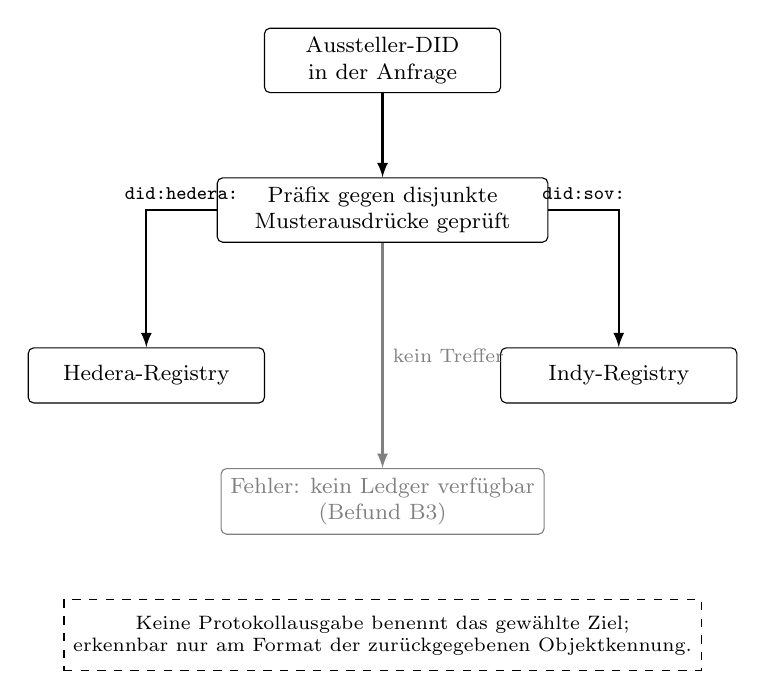
\begin{tikzpicture}[
      font=\footnotesize,
      box/.style={draw, rounded corners=2pt, minimum width=3.0cm, minimum height=0.7cm, align=center},
      pfeil/.style={-latex, thick}
    ]
      \node[box] (did) at (0,0) {Aussteller-DID\\ in der Anfrage};
      \node[box, minimum width=4.2cm] (test) at (0,-1.9) {Präfix gegen disjunkte\\ Musterausdrücke geprüft};
      \node[box] (hedera) at (-3.0,-4.0) {Hedera-Registry};
      \node[box] (indy) at (3.0,-4.0) {Indy-Registry};
      \node[box, draw=gray, text=gray] (fehler) at (0,-5.6) {Fehler: kein Ledger verfügbar\\ (Befund B3)};
      \draw[pfeil] (did) -- (test);
      \draw[pfeil] (test) -| node[above, pos=0.25, font=\scriptsize] {\texttt{did:hedera:}} (hedera);
      \draw[pfeil] (test) -| node[above, pos=0.25, font=\scriptsize] {\texttt{did:sov:}} (indy);
      \draw[pfeil, gray] (test) -- node[right, font=\scriptsize] {kein Treffer} (fehler);
      \node[draw, dashed, align=center, font=\scriptsize, minimum height=0.9cm] (log) at (0,-7.3) {Keine Protokollausgabe benennt das gewählte Ziel;\\ erkennbar nur am Format der zurückgegebenen Objektkennung.};
    \end{tikzpicture}
    \caption{Auswahl der Registry-Implementierung allein anhand des Präfixes der Aussteller-DID. Die gewählte Ledger-Variante geht aus keiner Protokollausgabe hervor; diese Nichtbeobachtbarkeit ist selbst der Befund (B2) und erzwingt für jede Messung einen Nachweis der tatsächlich angesprochenen Variante über die Objektkennung.}
    \label{fig:impl-dispatch}
\end{figure}


\section{Gültigkeitsgrenzen der Umsetzung}
\label{sec:impl-grenzen}

Die folgenden Grenzen ergeben sich aus der Umsetzung selbst und ergänzen die bereits im Evaluationskonzept festgehaltenen Grenzen (Abschnitt~\ref{subsec:eval-validitaet}).

\begin{itemize}
  \item Beide Varianten werden auf einem einzelnen Rechner betrieben. Die Konsens- und Validatorknoten teilen sich damit Prozessor, Arbeitsspeicher und Datenträger; Netzwerklaufzeiten zwischen den Knoten treten praktisch nicht auf. Absolute Latenzwerte sind deshalb nicht auf verteilt betriebene Netzwerke übertragbar. Da diese Bedingung für beide Varianten gleichermaßen gilt, bleibt der Vergleich zwischen ihnen davon unberührt.
  \item Das eingesetzte Bereitstellungswerkzeug erzeugt eine Entwicklungskonfiguration und keine Produktivkonfiguration. Sie eignet sich für den kontrollierten Vergleich, nicht jedoch für Aussagen über die im Produktivbetrieb erreichbare Leistung.
  \item Der Messaufbau enthält die Anwendungskomponenten der Referenzarchitektur nicht. Die gemessenen Werte beschreiben die Ledger-Schicht, nicht die von einem Endanwender wahrgenommene Antwortzeit des Gesamtsystems.
  \item Die in Abschnitt~\ref{sec:impl-symmetrie} beschriebene Rückstufung einer kryptografischen Basisbibliothek ist die einzige verbliebene, nicht auflösbare Abweichung zwischen den beiden Varianten.
  \item Die Indy-Variante wurde im Verlauf der Arbeit deutlich weniger häufig aufgebaut und betrieben als die HCS-Variante. Beobachtungen zu Betriebsverhalten und Fehlerarten sind daher für die Indy-Variante weniger breit abgesichert; für die eigentlichen Messwerte ist dies ohne Bedeutung, da beide Varianten unter demselben Messprotokoll erhoben werden.
  \item Die genaue Leseregel der eingesetzten Indy-Klientbibliothek, insbesondere die Anzahl der für eine Leseantwort herangezogenen Knoten, ließ sich aus der verfügbaren Dokumentation nicht abschließend bestimmen. Aussagen über das Leseverhalten der Indy-Variante bei Knotenausfall werden deshalb ausschließlich auf beobachtetes Verhalten und nicht auf eine dokumentierte Regel gestützt.
  \item Der Stand der Indy-Knoten ist ausschließlich über ein veränderliches Abbild-Kennzeichen festgehalten, nicht über einen Prüfwert oder einen Commit-Stand (Abschnitt~\ref{subsec:impl-indy-netzwerk}). Ein späterer Nachbau anhand der dokumentierten Angaben erzeugt daher nicht mit Sicherheit dasselbe Knotenabbild. Alle berichteten Messungen wurden gegen denselben, einmal erzeugten Abbildstand ausgeführt, sodass der Vergleich selbst davon unberührt bleibt; die Wiederholbarkeit der Messung durch Dritte ist jedoch eingeschränkt.
  \item Die Zuordnung der Schreibrolle zur DID des Agenten entsteht beim erstmaligen Hochfahren des Indy-Netzwerks und liegt nicht als Konfigurationsangabe im Messaufbau vor. Sie ist deshalb über das beobachtete Verhalten des Ledgers belegt und nicht über eine hinterlegte Festlegung.
  \item Die absoluten Ausfall- und Wiederherstellungsdauern des Szenarios S4 sind zwischen den Varianten nur eingeschränkt vergleichbar, da der Ausfall mit unterschiedlichen Mitteln herbeigeführt wird und auf der HCS-Variante ein erheblicher Anteil der gemessenen Dauer auf die Ausführungszeit der Verwaltungsbefehle entfällt (Abschnitt~\ref{sec:impl-szenarien}). Vergleichbar sind die Verlaufsform und die Richtung des Effekts, nicht die Absolutwerte.
  \item Die Prüfungen des Szenarios S5 und die Messung des Widerrufspfads werden unterhalb des Agenten über direkte Ledger-Aufrufe geführt (Abschnitt~\ref{subsec:impl-szenario-s5}). Ihre Ergebnisse beschreiben deshalb das Verhalten der Ledger-Schicht und nicht dasjenige des im Betrieb üblichen Zugriffswegs über die Agentenschicht.
\end{itemize}


\section{Zusammenfassung}
\label{sec:impl-zusammenfassung}

Dieses Kapitel hat den Aufbau beschrieben, mit dem die im Evaluationskonzept festgelegten Szenarien durchgeführt werden. Umgesetzt sind zwei Varianten mit identisch konfigurierter Agentenschicht und je vier Ledger-Knoten, deren Messgrenze durch den Vergleich der registrierten Schnittstellen am laufenden System als symmetrisch nachgewiesen wurde. Die HCS-Variante erforderte dabei drei über die reine Konfiguration hinausgehende Eingriffe: den mehrschrittigen Netzwerkaufbau anstelle des fehlerhaften Einschrittbefehls, die Anhebung einer zu niedrig gesetzten Speicherobergrenze und eine auf die Validierungsebene beschränkte Anpassung der DID-Bibliothek.

Der methodisch aufwendigste Teil betrifft nicht den Aufbau, sondern die Zeitnahme. Da der Konsens-Zeitstempel und die lokale Messuhr nicht vergleichbar sind, wird der Abstand zwischen Konsens und Abrufbarkeit als Intervall aus einer Zeitklammer bestimmt statt als Punktwert. Da die Sichtbarkeit zudem an den Abschluss von Aufzeichnungsdateien gebunden und damit quantisiert ist, wird jeder Einzelwert in einen Phasen- und einen Verarbeitungsanteil zerlegt und nur der Verarbeitungsanteil in den Vergleich eingesetzt. Beides zusammen macht aus einer stark streuenden Rohgröße eine belastbare Vergleichsgröße; die zugehörigen Werte werden in Kapitel~\ref{sec:results} berichtet.

Neben dem Aufbau sind sieben strukturelle Befunde entstanden, die keine Messwerte sind. Drei von ihnen betreffen die Beobachtbarkeit: Der Wallet-Typ entscheidet ohne Warnung über die Verfügbarkeit der Arbeitsschnittstellen, die Auswahl der Ledger-Variante erfolgt allein anhand des DID-Präfixes, ohne dass eine Protokollausgabe das gewählte Ziel benennt, und eine Fehlkonfiguration meldet sich als Verfügbarkeitsproblem der Infrastruktur. Zwei weitere betreffen das Verhältnis von Technologie und Klientbibliothek: ein fest ausgewartetes Zeitfenster auf dem Lesepfad und ein fehlendes Wiederholungsverhalten bei vorübergehender Ablehnung auf dem Schreibpfad. Die verbleibenden zwei betreffen die Schreibkontrolle -- ihre kategoriale Verschiedenheit zwischen beiden Varianten und der Umstand, dass beide Modelle durch die darüberliegende Agentenschicht in gleicher Weise unterlaufen werden können.

Der letztgenannte Befund hat unmittelbar die Anlage der Messungen bestimmt: Die Prüfungen der Zugriffskontrolle und die Messung des Widerrufspfads werden aus diesem Grund nicht über die Verwaltungsschnittstelle des Agenten, sondern unterhalb davon über direkte Ledger-Aufrufe geführt. Die berichteten Ergebnisse sind damit Aussagen über die Ledger-Schicht und nicht über den Weg, den eine Anwendung im Betrieb nehmen würde. Diese Befunde bilden zusammen mit den in Kapitel~\ref{sec:results} berichteten Messwerten die Grundlage der Diskussion in Kapitel~\ref{sec:discussion}.